\section{Branching ratios\footnote{A.~Denner, S.~Heinemeyer,
    I.~Puljak, D.~Rebuzzi (eds.); S. Dittmaier, A. M\"uck, M. Spira,
    M. Weber and G. Weiglein.}}

%\vspace{0.5cm}
%\leftline{{\em Working group}:
%A.~Denner, S.~Heinemeyer, I.~Puljak, D.~Rebuzzi,}
%\leftline{\qquad\qquad S. Dittmaier, A. M\"uck, M. Spira, M. Weber, G. Weiglein}
%\vspace{0.2cm}

\label{sec:BR}


\subsection{Standard Model (SM) Higgs branching ratios}
\label{sec:SM-BR}
%%% Ansgar

\providecommand{\lsim}
{\;\raisebox{-.3em}{$\stackrel{\displaystyle <}{\sim}$}\;}
\providecommand{\gsim}
{\;\raisebox{-.3em}{$\stackrel{\displaystyle >}{\sim}$}\;}

%\renewcommand{\MH}{M_{\PH}}

%\newcommand{\dtm}[1]{\cdot 10^{-#}}
%\newcommand{\dtp}[1]{\cdot 10^{#}}
%--
\providecommand{\HDECAY}{{\sc HDECAY}}
\providecommand{\HIGLU}{{\sc HIGLU}}
\providecommand{\Prophecy}{{\sc Prophecy4f}}
\providecommand{\CPsuperH}{{\sc CPsuperH}}
\providecommand{\FeynHiggs}{{\sc FeynHiggs}}


The branching ratios of the Higgs boson in the Standard Model have
been determined using the programs {\sc HDECAY}
\cite{Djouadi:1997yw,Spira:1997dg,hdecay2}
and {\sc Prophecy4f}
\cite{Bredenstein:2006rh,Bredenstein:2006ha,Prophecy4f}. In a first
step, all partial widths have been calculated as accurately as
possible. Then the branching ratios have been derived from this full
set of partial widths. Since the widths are calculated for on-shell
Higgs bosons, the results have to be used with care for a heavy Higgs
boson ($\MH\gsim500\UGeV$).

The code {\sc HDECAY} calculates the decay widths and branching ratios
of the Higgs boson(s) in the SM and the MSSM. For the SM it includes
all kinematically allowed channels and all relevant higher-order
QCD corrections to decays into quark pairs and into gluons. More
details are given below.
%
The electroweak next-to-leading order (NLO)
corrections to the decays $\PH\to\PGg\PGg$ and
$\PH\to \Pg\Pg$ have been calculated in
\Brefs{Aglietti:2004ki,Aglietti:2004nj,Aglietti:2006ne,Degrassi:2004mx,Degrassi:2005mc,Actis:2008ug}.
They are implemented in {\sc HDECAY} in form of a grid based on the
calculation of \Bref{Actis:2008ug}.


{\sc Prophecy4f} is a Monte Carlo event generator for $\PH \to
\PW\PW/\PZ\PZ \to 4f$ (leptonic, semi-leptonic, and hadronic)
final states. It provides the leading-order (LO) and NLO partial widths for any
possible 4-fermion final state. It includes the complete NLO QCD and
electroweak corrections and all interferences at LO and NLO. In other
words, it takes into account both the corrections to the decays into
intermediate $\PW\PW$ and $\PZ\PZ$ states as well as their
interference for final states that allow for both. The dominant two-loop
contributions in the heavy-Higgs-mass limit proportional to $G_\mu^2
\MH^4$ are included according to \Brefs{Ghinculov:1995bz,Frink:1996sv}.
Since the calculation is consistently performed with off-shell gauge
bosons without any on-shell approximation, it is valid above, near,
and below the gauge-boson pair thresholds. Like all other light quarks
and leptons, bottom quarks are treated as massless.  Using the LO/NLO
gauge-boson widths in the LO/NLO calculation ensures that the
effective branching ratios of the $\PW$ and $\PZ$ bosons obtained by summing
over all decay channels add up to one.

The results presented below have been obtained as follows. The Higgs total
width resulting from {\sc HDECAY} has been modified according to the
prescription
\begin{equation}
\Gamma_{\PH}=\Gamma^{\mathrm{HD}}-\Gamma^{\mathrm{HD}}_{\PZ\PZ}-\Gamma^{\mathrm{HD}}_{\PW\PW}+\Gamma^{\mathrm{Proph.}}_{4f}
%+\Ga^{\mathrm{HD}}_{\ga\ga}
%(\de^{\mathrm{EW}}_{\ga\ga}+
%\de^{\mathrm{QED}}_{\ga f f}
%)
,
\end{equation}
where $\Gamma_{\PH}$ is the total Higgs width, $\Gamma^{\mathrm{HD}}$
the Higgs width obtained from {\sc HDECAY},
$\Gamma^{\mathrm{HD}}_{\PZ\PZ}$ and $\Gamma^{\mathrm{HD}}_{\PW\PW}$
stand for the partial widths to $\PZ\PZ$ and $\PW\PW$ calculated with
{\sc HDECAY}, while $\Gamma^{\mathrm{Proph.}}_{4f}$ represents the
partial width of $\PH\to 4f$ calculated with {\sc Prophecy4f}.  The
latter can be split into the decays into $\PZ\PZ$, $\PW\PW$, and the
interference,
\begin{equation}
\Gamma^{\mathrm{Proph.}}_{4f}=\Gamma_{{\mathrm{H}}\to \PW^*\PW^*\to 4f}
+ \Gamma_{{\mathrm{H}}\to \PZ^*\PZ^*\to 4f}
+ \Gamma_{\mathrm{\PW\PW/\PZ\PZ-int.}}.
\end{equation}

The relative theoretical uncertainties of the calculation resulting
from  missing higher-order corrections are summarized in \refT{tab:uncertainty}.

\begin{table}[ht]
   \caption{Estimate of theoretical uncertainties from missing higher orders.}
   \begin{center}
   \small  
   \begin{tabular}{lllll}
   \hline
   \textbf{Partial width} & \textbf{QCD} & \textbf{Electroweak} & \textbf{Total} \\
\hline
 $\PH \to \PQb\PQb/\PQc\PQc$ &    $\sim 0.1{-}0.2\%$
  &     $\sim 1$--$2\%$ for $\MH \lsim 135\UGeV$     &      $\sim1$--$2 \%$ \\
\hline
$\PH\to \PGt \PGt$ & & $\sim1$--$2\%$  for $\MH \lsim 135\UGeV$ &       $\sim1$--$2 \%$ \\
\hline
$\PH \to \PQt\PQt$ & $\sim 5\%$&
      ${\lsim  2}$--${5\%}$   for $\MH < 500\UGeV$     &       $\sim5\%$ \\
& &      $\sim 0.1 ({\MH}/{1\UTeV})^4$ for $\MH > 500\UGeV$  &       $\sim5$--$10\%$ \\
\hline
$\PH \to \Pg\Pg$ & ${\sim 10\%}$   &
$\sim 1\%$   &   $\sim10\%$\\
\hline
$\PH \to \PGg \PGg$  & ${<1\%}$ & $<1\%$    &  $\sim1\%$ \\
\hline
$\PH \to \PW\PW/\PZ\PZ\to4f$ & $<0.5\%$ &   $\sim 0.5\%$ for $\MH < 500\UGeV$ &  $\sim0.5\%$\\
$\phantom{\PH\to    \to 4f}$             && $\sim 0.17 ({\MH}/{1\UTeV})^4$ for $\MH > 500\UGeV$
&        $\sim0.5$--$15\%$                          \\
\hline
\end{tabular}
\end{center}
\label{tab:uncertainty}
\end{table}
%Note that this does not include parametric uncertainties.
For QCD corrections the uncertainties have been estimated by
the scale dependence of the widths resulting from a  variation of the scale
up and down by a factor $2$ or from the size of known omitted
corrections. For electroweak corrections the missing higher orders
have been estimated based on the known structure and size of the NLO
corrections. For cases where HDECAY takes into account the known NLO
corrections only approximately the accuracy of these approximations
has been used.
These theoretical uncertainties from missing higher-order corrections will
have to be combined with the parametric uncertainties (most notably from the
bottom-quark mass and $\alphas$) to arrive at the full theory uncertainties.

Specifically, the uncertainties of the results from \HDECAY\ are
obtained as follows: For the decays $\PH \to \PQb\PQb, \PQc\PQc$,
\HDECAY\ includes the complete massless QCD corrections up to and
including NNNLO, with a corresponding scale dependence of about
$0.1{-}0.2\%$. The NLO electroweak corrections
\cite{Fleischer:1980ub,Bardin:1990zj,Dabelstein:1991ky,Kniehl:1991ze}
are included in the approximation for small Higgs masses
\cite{Accomando:1997wt} which has an accuracy of about $1\%$ for $\MH <
135\UGeV$.  The same applies to the electroweak corrections to $\PH \to
\PGtp \PGtm$.  For Higgs decays into top quarks \HDECAY\ includes
the complete NLO QCD corrections for small Higgs masses
\cite{Braaten:1980yq,Sakai:1980fa,Inami:1980qp,Gorishnii:1983cu,Drees:1989du,Drees:1990dq,Drees:1991dq}
interpolated to the large-Higgs-mass results at NNNLO far above the
threshold
\cite{Gorishnii:1990zu,Gorishnii:1991zr,Kataev:1993be,Surguladze:1994gc,Larin:1995sq,Chetyrkin:1995pd,Chetyrkin:1996sr}.
The corresponding scale dependence is below $5\%$.  Only the NLO
electroweak corrections due to the self-interaction of the Higgs boson
are included, and the neglected electroweak corrections amount to
about $2{-}5\%$ for $\MH < 500\UGeV$, where $5\%$ refers to the region near
the $\PQt\bar\PQt$ threshold and $2\%$ to Higgs masses far above.  For
$\MH > 500$\UGeV\ higher-order heavy-Higgs corrections
\cite{Ghinculov:1994se,Ghinculov:1995err,Durand:1994pk,Durand:1994err,Durand:1994pw,Borodulin:1996br}
dominate the error, resulting in an uncertainty of
$0.1\times(\MH/1\UTeV)^4$ for $\MH > 500\UGeV$.  For $\PH \to \Pg\Pg$,
\HDECAY\ uses the NLO \cite{Inami:1982xt,Djouadi:1991tka,Spira:1995rr}
and NNLO \cite{Chetyrkin:1997iv} QCD corrections in the limit of heavy
top quarks, while NNNLO QCD corrections \cite{Baikov:2006ch} are
neglected.  The uncertainty from the scale dependence at NNLO is about
$10\%$ for $\MH < 135$\UGeV. The NLO electroweak corrections are included
via an interpolation based on a grid from \Bref{Actis:2008ug}; the
uncertainty from missing higher-order electroweak corrections is
estimated to be $1\%$.  For the decay $\PH\to\PGg \PGg$, \HDECAY\
includes the full NLO QCD corrections
\cite{Zheng:1990qa,Djouadi:1990aj,Dawson:1992cy,Djouadi:1993ji,Melnikov:1993tj,Inoue:1994jq,Spira:1995rr}
and a grid from \Bref{Actis:2008ug} for the NLO electroweak corrections.
Missing higher orders are estimated to be below $1\%$. The contribution of
the $\PH \rightarrow \PGg \Pe^{+}\Pe^{-}$ decay via virtual photon conversion,
evaluated in \Bref{Firan:2007tp} is not taken into account in the following results. Its correct treatment and its inclusion in HDECAY are in progress.


The decays $\PH \to \PW\PW/\PZ\PZ\to4f$ are based on \Prophecy, which
includes the complete NLO QCD and electroweak corrections with all
interferences and leading two-loop heavy-Higgs corrections.  For $\MH >
500$\UGeV\ higher-order heavy-Higgs corrections dominate the error
leading to an uncertainty of $0.17\times(\MH/1\UTeV)^4$ for $\MH >
500$\UGeV.

The assessment of parametric uncertainties of the Higgs branching ratios is still
work in progress. A thorough, but very conservative estimation has recently
been made in \Bref{Baglio:2010ae}.

%%%%%%%%%%%%%%%%%%%%%%%%%%%%%%%%%%%%%%%%%%%%%%%%%%%%%%%%%%%%%%%%%%%%%%%%%%%%%%
%%%%%%%%%%%%%%%%%%%%%%%%%%%%%%%%%%%%%%%%%%%%%%%%%%%%%%%%%%%%%%%%%%%%%%%%%%%%%%

\subsection{MSSM Higgs branching ratios: work in progress}
\label{sec:MSSM-BR}
\providecommand{\PA}{\mathrm{A}}
%\providecommand{\Mh}{\MH}
\providecommand{\MA}{M_{\PA}}
\newcommand{\tb}{\tan\beta}
\newcommand{\order}[1]{\ensuremath{{\cal O}(#1)}}
\newcommand{\mhmax}{\ensuremath{m_h^{\rm max}}}

The common issues of MSSM cross section and branching-ratio calculations
have been outlined in Section~\ref{sec:mssmvssm}.
It was stressed that {\em before} any branching-ratio calculation can be
performed in a first step the Higgs-boson masses, couplings, and mixings
have to be determined from the underlying set of (soft SUSY-breaking)
parameters. A brief comparison of the dedicated codes that provide this kind of
calculations
(\FeynHiggs~\cite{Heinemeyer:1998yj,Heinemeyer:1998np,Degrassi:2002fi,Frank:2006yh}
and \CPsuperH~\cite{Lee:2003nta,Lee:2007gn}) has been given, where in
the case of real parameters more corrections are included into
\FeynHiggs.

After the calculation of Higgs-boson masses and mixings from the
original SUSY input the branching-ratio calculation has to be
performed.  This can be done with the codes, \CPsuperH\ and
\FeynHiggs\ for real or complex parameters, or
\HDECAY~\cite{Djouadi:1997yw,Spira:1997dg,hdecay2} for real
parameters. The higher-order corrections included
in the calculation of the various decay channels differ in the three
codes. A detailed analysis of the accuracy of the different codes for
certain decay widths is currently performed.

As for MSSM Higgs-boson production cross sections (see
\Sref{sec:mssmvssm}) due to the
complexity of the MSSM parameter space, results can only be derived
in representative benchmark scenarios. In accordance with
\Sref{sec:mssm_neutral}
we show in \Tref{tab:BR-mssm} exemplary values for the
BR($\phi \to \PGtp\PGtm$) ($\phi = \Ph, \PH, \PA$),
in the $m_{\Ph}^{\rm max}$ scenario~\cite{Carena:2002qg}
(see Eq.~(\ref{YRHXS_MSSM_neutral_eq:mhmax}) for the definition of the SUSY
parameters) consistently derived
with \FeynHiggs\,2.7.4. In the further progress of this work a machinery will
be set up to evaluate MSSM Higgs-boson branching ratios (consistent with the
corresponding cross-section calculations) that will be valid for the full
MSSM parameter space.


\subsection{Results}

Final SM Higgs-boson branching ratios\footnote{Full listings can be found at
  {\sl https://twiki.cern.ch/twiki/bin/view/LHCPhysics/CERNYellowReportPageBR}}
for $2$-fermion final states,
gauge-boson pair and the total decay width are listed
in \Trefs{tab:BR-lm.part1}--\ref{tab:BR-hm.part2}.
In \Trefs{tab:PBR-lm}--\ref{tab:PBR-hm2} we list branching
ratios of the SM Higgs boson decaying into $4$-fermion final states,
where leptons $\Pl=\Pe,\PGm,\PGt,\PGn_{\Pe},\PGn_{\PGm},\PGn_{\PGt}$, 
and quarks $\PQq=\PQu,\PQd,\PQs,\PQc,\PQb$. 
All fermion masses are neglected, the branching ratios are therefore
identical for different flavours.
We display results for $4$-lepton final states ($\PH \to
\Pl\Pl\Pl\Pl$) in \Trefs{tab:PBR-lm}--\ref{tab:PBR-hm}. 
We also provide results for final states with $2$ arbitrary leptons
and quarks ($\PH \to \Pl\Pl\PQq\PQq$),
$4$ arbitrary quarks ($\PH \to \PQq\PQq\PQq\PQq$),
and for all possible $4$-fermion final states ($\PH \to \Pf\Pf\Pf\Pf$)
in \Trefs{tab:PBR-lm2}--\ref{tab:PBR-hm2}. 
For Higgs-boson masses below the
$\PZ\PZ$ threshold, interference contributions become relevant for $4$-fermion decays with identical
fermions like $\PH\to\PZ\PZ\to\Pe\Pe\Pe\Pe$ or
$\PH\to\PW\PW/\PZ\PZ\to\Pe\PGn_{\Pe}\Pe\PGn_{\Pe}$. These enhance
the branching ratios for $\PH \to
\Pe\Pe\Pe\Pe,\PGm\PGm\PGm\PGm$ by more than
$10\%$ and decrease those for
$\PH\to\Pe\PGn_{\Pe}\Pe\PGn_{\Pe}, \PGm\PGn_{\PGm}\PGm\PGn_{\PGm}$
by more than $5\%$ compared to those without identical fermions for
$\MH=120\UGeV$.
All partial widths are listed in Appendix~\ref{brappendix}.
%Corresponding Higgs-decay partial-widths are listed in \Trefs{tab:PWidth-lm}--\ref{tab:PWidth-hm2}.
Branching ratios as a function of the SM Higgs-boson mass up to $200\UGeV$ are shown in Fig.~\ref{fig:SMBR200}. The full mass range is displayed in Fig.~\ref{fig:SMBRs}. Figure~\ref{fig:SMWidth} shows the SM Higgs-boson total decay width as a function of its mass. 

MSSM Higgs-boson branching ratios to $\PGtp\PGtm$ final states in the
$m_{\Ph}^{\rm max}$ scenario as a function of $\MA$ [GeV] and $\tb$ are given
in Table~\ref{tab:BR-mssm} as an example of the MSSM results.

All results have been obtained using the values of the electroweak parameters as given in Appendix A. For the strong coupling constant we used $\alphas(\MZ^2) = 0.119$ with two-loop running.

% -------------------------------------

\begin{figure}[h]
  \centering\includegraphics[width=.70\linewidth]{YRHXS_BR/YRHXS_BR_fig1.eps}
  \caption{SM Higgs branching ratios as a function of the Higgs-boson mass.}
  \label{fig:SMBR200}
\end{figure}

\begin{figure}[h]
\centering\includegraphics[width=.70\linewidth]{YRHXS_BR/YRHXS_BR_fig2.eps}
\caption{SM Higgs total width  as a function of the Higgs-boson mass.}
\label{fig:SMWidth}
\end{figure}

% -------------------------------------

\begin{table}
%  \thisfloatpagestyle{empty}
  \vspace{-\headsep}
  \caption{SM Higgs branching ratios in fermionic final states in the low-
  and intermediate-mass range.}
  \label{tab:BR-lm.part1}
  \centering
%  \renewcommand{\arraystretch}{0.92}
  \small
  \begin{tabular}{lcccccc}\hline
$\MH$ [GeV] & $\PH \rightarrow \PQb\PAQb$ & $\PH \rightarrow \PGt \PGt$ & $\PH \rightarrow
\PGm \PGm$ & $\PH \rightarrow \PQs \PAQs$ & $\PH \rightarrow \PQc \PAQc$
& $\PH \rightarrow \PQt \PAQt$ \\
\hline
$90 $&$ 8.12\cdot 10^{-1}  $&$ 8.41\cdot 10^{-2}  $&$ 2.92\cdot 10^{-4}  $&$ 6.20\cdot 10^{-4}  $&$ 3.78\cdot 10^{-2}  $&$ 0.00 $\\
$95 $&$ 8.04\cdot 10^{-1}  $&$ 8.41\cdot 10^{-2}  $&$ 2.92\cdot 10^{-4}  $&$ 6.13\cdot 10^{-4}  $&$ 3.73\cdot 10^{-2}  $&$ 0.00 $\\
$100 $&$ 7.91\cdot 10^{-1}  $&$ 8.36\cdot 10^{-2}  $&$ 2.90\cdot 10^{-4}  $&$ 6.03\cdot 10^{-4}  $&$ 3.68\cdot 10^{-2}  $&$ 0.00 $\\
$105 $&$ 7.73\cdot 10^{-1}  $&$ 8.25\cdot 10^{-2}  $&$ 2.86\cdot 10^{-4}  $&$ 5.89\cdot 10^{-4}  $&$ 3.59\cdot 10^{-2}  $&$ 0.00 $\\
$110 $&$ 7.45\cdot 10^{-1}  $&$ 8.03\cdot 10^{-2}  $&$ 2.79\cdot 10^{-4}  $&$ 5.68\cdot 10^{-4}  $&$ 3.46\cdot 10^{-2}  $&$ 0.00 $\\
$115 $&$ 7.05\cdot 10^{-1}  $&$ 7.65\cdot 10^{-2}  $&$ 2.66\cdot 10^{-4}  $&$ 5.37\cdot 10^{-4}  $&$ 3.27\cdot 10^{-2}  $&$ 0.00 $\\
$120 $&$ 6.49\cdot 10^{-1}  $&$ 7.11\cdot 10^{-2}  $&$ 2.47\cdot 10^{-4}  $&$ 4.94\cdot 10^{-4}  $&$ 3.01\cdot 10^{-2}  $&$ 0.00 $\\
$125 $&$ 5.78\cdot 10^{-1}  $&$ 6.37\cdot 10^{-2}  $&$ 2.21\cdot 10^{-4}  $&$ 4.40\cdot 10^{-4}  $&$ 2.68\cdot 10^{-2}  $&$ 0.00 $\\
$130 $&$ 4.94\cdot 10^{-1}  $&$ 5.49\cdot 10^{-2}  $&$ 1.91\cdot 10^{-4}  $&$ 3.76\cdot 10^{-4}  $&$ 2.29\cdot 10^{-2}  $&$ 0.00 $\\
$135 $&$ 4.04\cdot 10^{-1}  $&$ 4.52\cdot 10^{-2}  $&$ 1.57\cdot 10^{-4}  $&$ 3.07\cdot 10^{-4}  $&$ 1.87\cdot 10^{-2}  $&$ 0.00 $\\
$140 $&$ 3.14\cdot 10^{-1}  $&$ 3.54\cdot 10^{-2}  $&$ 1.23\cdot 10^{-4}  $&$ 2.39\cdot 10^{-4}  $&$ 1.46\cdot 10^{-2}  $&$ 0.00 $\\
$145 $&$ 2.31\cdot 10^{-1}  $&$ 2.62\cdot 10^{-2}  $&$ 9.09\cdot 10^{-5}  $&$ 1.76\cdot 10^{-4}  $&$ 1.07\cdot 10^{-2}  $&$ 0.00 $\\
$150 $&$ 1.57\cdot 10^{-1}  $&$ 1.79\cdot 10^{-2}  $&$ 6.20\cdot 10^{-5}  $&$ 1.19\cdot 10^{-4}  $&$ 7.25\cdot 10^{-3}  $&$ 0.00 $\\
$155 $&$ 9.18\cdot 10^{-2}  $&$ 1.06\cdot 10^{-2}  $&$ 3.66\cdot 10^{-5}  $&$ 6.98\cdot 10^{-5}  $&$ 4.25\cdot 10^{-3}  $&$ 0.00 $\\
$160 $&$ 3.44\cdot 10^{-2}  $&$ 3.97\cdot 10^{-3}  $&$ 1.38\cdot 10^{-5}  $&$ 2.61\cdot 10^{-5}  $&$ 1.59\cdot 10^{-3}  $&$ 0.00 $\\
$165 $&$ 1.19\cdot 10^{-2}  $&$ 1.38\cdot 10^{-3}  $&$ 4.78\cdot 10^{-6}  $&$ 9.02\cdot 10^{-6}  $&$ 5.49\cdot 10^{-4}  $&$ 0.00 $\\
$170 $&$ 7.87\cdot 10^{-3}  $&$ 9.20\cdot 10^{-4}  $&$ 3.19\cdot 10^{-6}  $&$ 5.99\cdot 10^{-6}  $&$ 3.64\cdot 10^{-4}  $&$ 0.00 $\\
$175 $&$ 6.12\cdot 10^{-3}  $&$ 7.19\cdot 10^{-4}  $&$ 2.49\cdot 10^{-6}  $&$ 4.65\cdot 10^{-6}  $&$ 2.83\cdot 10^{-4}  $&$ 0.00 $\\
$180 $&$ 4.97\cdot 10^{-3}  $&$ 5.87\cdot 10^{-4}  $&$ 2.04\cdot 10^{-6}  $&$ 3.78\cdot 10^{-6}  $&$ 2.30\cdot 10^{-4}  $&$ 0.00 $\\
$185 $&$ 3.85\cdot 10^{-3}  $&$ 4.57\cdot 10^{-4}  $&$ 1.59\cdot 10^{-6}  $&$ 2.93\cdot 10^{-6}  $&$ 1.78\cdot 10^{-4}  $&$ 0.00 $\\
$190 $&$ 3.15\cdot 10^{-3}  $&$ 3.76\cdot 10^{-4}  $&$ 1.30\cdot 10^{-6}  $&$ 2.39\cdot 10^{-6}  $&$ 1.46\cdot 10^{-4}  $&$ 0.00 $\\
$195 $&$ 2.70\cdot 10^{-3}  $&$ 3.24\cdot 10^{-4}  $&$ 1.13\cdot 10^{-6}  $&$ 2.06\cdot 10^{-6}  $&$ 1.25\cdot 10^{-4}  $&$ 0.00 $\\
$200 $&$ 2.38\cdot 10^{-3}  $&$ 2.87\cdot 10^{-4}  $&$ 9.96\cdot 10^{-7}  $&$ 1.81\cdot 10^{-6}  $&$ 1.10\cdot 10^{-4}  $&$ 0.00 $\\
$210 $&$ 1.92\cdot 10^{-3}  $&$ 2.34\cdot 10^{-4}  $&$ 8.11\cdot 10^{-7}  $&$ 1.46\cdot 10^{-6}  $&$ 8.89\cdot 10^{-5}  $&$ 0.00 $\\
$220 $&$ 1.60\cdot 10^{-3}  $&$ 1.96\cdot 10^{-4}  $&$ 6.81\cdot 10^{-7}  $&$ 1.22\cdot 10^{-6}  $&$ 7.40\cdot 10^{-5}  $&$ 0.00 $\\
$230 $&$ 1.36\cdot 10^{-3}  $&$ 1.68\cdot 10^{-4}  $&$ 5.82\cdot 10^{-7}  $&$ 1.03\cdot 10^{-6}  $&$ 6.27\cdot 10^{-5}  $&$ 0.00 $\\
$240 $&$ 1.17\cdot 10^{-3}  $&$ 1.45\cdot 10^{-4}  $&$ 5.04\cdot 10^{-7}  $&$ 8.86\cdot 10^{-7}  $&$ 5.39\cdot 10^{-5}  $&$ 0.00 $\\
$250 $&$ 1.01\cdot 10^{-3}  $&$ 1.27\cdot 10^{-4}  $&$ 4.42\cdot 10^{-7}  $&$ 7.70\cdot 10^{-7}  $&$ 4.68\cdot 10^{-5}  $&$ 0.00 $\\
$260 $&$ 8.89\cdot 10^{-4}  $&$ 1.12\cdot 10^{-4}  $&$ 3.90\cdot 10^{-7}  $&$ 6.75\cdot 10^{-7}  $&$ 4.11\cdot 10^{-5}  $&$ 5.14\cdot 10^{-8}  $\\
$270 $&$ 7.86\cdot 10^{-4}  $&$ 1.00\cdot 10^{-4}  $&$ 3.47\cdot 10^{-7}  $&$ 5.97\cdot 10^{-7}  $&$ 3.63\cdot 10^{-5}  $&$ 2.29\cdot 10^{-6}  $\\
$280 $&$ 7.00\cdot 10^{-4}  $&$ 8.98\cdot 10^{-5}  $&$ 3.11\cdot 10^{-7}  $&$ 5.31\cdot 10^{-7}  $&$ 3.23\cdot 10^{-5}  $&$ 1.09\cdot 10^{-5}  $\\
$290 $&$ 6.27\cdot 10^{-4}  $&$ 8.09\cdot 10^{-5}  $&$ 2.80\cdot 10^{-7}  $&$ 4.76\cdot 10^{-7}  $&$ 2.90\cdot 10^{-5}  $&$ 3.06\cdot 10^{-5}  $\\
$300 $&$ 5.65\cdot 10^{-4}  $&$ 7.33\cdot 10^{-5}  $&$ 2.54\cdot 10^{-7}  $&$ 4.29\cdot 10^{-7}  $&$ 2.61\cdot 10^{-5}  $&$ 6.87\cdot 10^{-5}  $\\
$310 $&$ 5.12\cdot 10^{-4}  $&$ 6.68\cdot 10^{-5}  $&$ 2.32\cdot 10^{-7}  $&$ 3.89\cdot 10^{-7}  $&$ 2.36\cdot 10^{-5}  $&$ 1.38\cdot 10^{-4}  $\\
$320 $&$ 4.66\cdot 10^{-4}  $&$ 6.12\cdot 10^{-5}  $&$ 2.12\cdot 10^{-7}  $&$ 3.54\cdot 10^{-7}  $&$ 2.15\cdot 10^{-5}  $&$ 2.66\cdot 10^{-4}  $\\
$330 $&$ 4.26\cdot 10^{-4}  $&$ 5.63\cdot 10^{-5}  $&$ 1.95\cdot 10^{-7}  $&$ 3.24\cdot 10^{-7}  $&$ 1.97\cdot 10^{-5}  $&$ 5.21\cdot 10^{-4}  $\\
$340 $&$ 3.92\cdot 10^{-4}  $&$ 5.20\cdot 10^{-5}  $&$ 1.80\cdot 10^{-7}  $&$ 2.98\cdot 10^{-7}  $&$ 1.81\cdot 10^{-5}  $&$ 1.20\cdot 10^{-3}  $\\
$350 $&$ 3.57\cdot 10^{-4}  $&$ 4.76\cdot 10^{-5}  $&$ 1.65\cdot 10^{-7}  $&$ 2.71\cdot 10^{-7}  $&$ 1.65\cdot 10^{-5}  $&$ 1.56\cdot 10^{-2}  $\\
$360 $&$ 3.16\cdot 10^{-4}  $&$ 4.23\cdot 10^{-5}  $&$ 1.47\cdot 10^{-7}  $&$ 2.40\cdot 10^{-7}  $&$ 1.46\cdot 10^{-5}  $&$ 5.15\cdot 10^{-2}  $\\
$370 $&$ 2.81\cdot 10^{-4}  $&$ 3.78\cdot 10^{-5}  $&$ 1.31\cdot 10^{-7}  $&$ 2.13\cdot 10^{-7}  $&$ 1.29\cdot 10^{-5}  $&$ 8.37\cdot 10^{-2}  $\\
$380 $&$ 2.52\cdot 10^{-4}  $&$ 3.40\cdot 10^{-5}  $&$ 1.18\cdot 10^{-7}  $&$ 1.91\cdot 10^{-7}  $&$ 1.16\cdot 10^{-5}  $&$ 1.10\cdot 10^{-1}  $\\
$390 $&$ 2.28\cdot 10^{-4}  $&$ 3.10\cdot 10^{-5}  $&$ 1.07\cdot 10^{-7}  $&$ 1.73\cdot 10^{-7}  $&$ 1.05\cdot 10^{-5}  $&$ 1.32\cdot 10^{-1}  $\\
$400 $&$ 2.08\cdot 10^{-4}  $&$ 2.84\cdot 10^{-5}  $&$ 9.83\cdot 10^{-8}  $&$ 1.58\cdot 10^{-7}  $&$ 9.59\cdot 10^{-6}  $&$ 1.48\cdot 10^{-1}  $\\
$410 $&$ 1.91\cdot 10^{-4}  $&$ 2.61\cdot 10^{-5}  $&$ 9.06\cdot 10^{-8}  $&$ 1.45\cdot 10^{-7}  $&$ 8.80\cdot 10^{-6}  $&$ 1.62\cdot 10^{-1}  $\\
$420 $&$ 1.76\cdot 10^{-4}  $&$ 2.43\cdot 10^{-5}  $&$ 8.41\cdot 10^{-8}  $&$ 1.34\cdot 10^{-7}  $&$ 8.13\cdot 10^{-6}  $&$ 1.72\cdot 10^{-1}  $\\
$430 $&$ 1.64\cdot 10^{-4}  $&$ 2.26\cdot 10^{-5}  $&$ 7.84\cdot 10^{-8}  $&$ 1.24\cdot 10^{-7}  $&$ 7.55\cdot 10^{-6}  $&$ 1.79\cdot 10^{-1}  $\\
$440 $&$ 1.53\cdot 10^{-4}  $&$ 2.12\cdot 10^{-5}  $&$ 7.34\cdot 10^{-8}  $&$ 1.16\cdot 10^{-7}  $&$ 7.05\cdot 10^{-6}  $&$ 1.85\cdot 10^{-1}  $\\
$450 $&$ 1.43\cdot 10^{-4}  $&$ 1.99\cdot 10^{-5}  $&$ 6.90\cdot 10^{-8}  $&$ 1.09\cdot 10^{-7}  $&$ 6.60\cdot 10^{-6}  $&$ 1.89\cdot 10^{-1}  $\\
$460 $&$ 1.35\cdot 10^{-4}  $&$ 1.88\cdot 10^{-5}  $&$ 6.51\cdot 10^{-8}  $&$ 1.02\cdot 10^{-7}  $&$ 6.21\cdot 10^{-6}  $&$ 1.91\cdot 10^{-1}  $\\
$470 $&$ 1.27\cdot 10^{-4}  $&$ 1.78\cdot 10^{-5}  $&$ 6.16\cdot 10^{-8}  $&$ 9.63\cdot 10^{-8}  $&$ 5.85\cdot 10^{-6}  $&$ 1.93\cdot 10^{-1}  $\\
$480 $&$ 1.20\cdot 10^{-4}  $&$ 1.69\cdot 10^{-5}  $&$ 5.85\cdot 10^{-8}  $&$ 9.10\cdot 10^{-8}  $&$ 5.53\cdot 10^{-6}  $&$ 1.94\cdot 10^{-1}  $\\
$490 $&$ 1.14\cdot 10^{-4}  $&$ 1.60\cdot 10^{-5}  $&$ 5.56\cdot 10^{-8}  $&$ 8.63\cdot 10^{-8}  $&$ 5.24\cdot 10^{-6}  $&$ 1.94\cdot 10^{-1}  $\\
\hline
  \end{tabular}
\end{table}

\begin{table}
%  \thisfloatpagestyle{empty}
  \vspace{-\headsep}
  \caption{SM Higgs branching ratios in fermionic final states in the high-mass range.}
  \label{tab:BR-hm.part1}
  \centering
%  \renewcommand{\arraystretch}{0.92}
  \small
  \begin{tabular}{lcccccc}\hline
$\MH$ [GeV] & $\PH \rightarrow \PQb\PAQb$ & $\PH \rightarrow \PGt \PGt$ & $\PH \rightarrow
\PGm \PGm$ & $\PH \rightarrow \PQs \PAQs$ & $\PH \rightarrow \PQc \PAQc$
& $\PH \rightarrow \PQt \PAQt$ \\
\hline
$500 $&$ 1.08\cdot 10^{-4}  $&$ 1.53\cdot 10^{-5}  $&$ 5.30\cdot 10^{-8}  $&$ 8.19\cdot 10^{-8}  $&$ 4.98\cdot 10^{-6}  $&$ 1.93\cdot 10^{-1}  $\\
$510 $&$ 1.03\cdot 10^{-4}  $&$ 1.46\cdot 10^{-5}  $&$ 5.06\cdot 10^{-8}  $&$ 7.80\cdot 10^{-8}  $&$ 4.74\cdot 10^{-6}  $&$ 1.92\cdot 10^{-1}  $\\
$520 $&$ 9.80\cdot 10^{-5}  $&$ 1.40\cdot 10^{-5}  $&$ 4.84\cdot 10^{-8}  $&$ 7.44\cdot 10^{-8}  $&$ 4.52\cdot 10^{-6}  $&$ 1.90\cdot 10^{-1}  $\\
$530 $&$ 9.36\cdot 10^{-5}  $&$ 1.34\cdot 10^{-5}  $&$ 4.64\cdot 10^{-8}  $&$ 7.10\cdot 10^{-8}  $&$ 4.31\cdot 10^{-6}  $&$ 1.88\cdot 10^{-1}  $\\
$540 $&$ 8.95\cdot 10^{-5}  $&$ 1.28\cdot 10^{-5}  $&$ 4.45\cdot 10^{-8}  $&$ 6.79\cdot 10^{-8}  $&$ 4.12\cdot 10^{-6}  $&$ 1.86\cdot 10^{-1}  $\\
$550 $&$ 8.57\cdot 10^{-5}  $&$ 1.23\cdot 10^{-5}  $&$ 4.27\cdot 10^{-8}  $&$ 6.50\cdot 10^{-8}  $&$ 3.95\cdot 10^{-6}  $&$ 1.84\cdot 10^{-1}  $\\
$560 $&$ 8.21\cdot 10^{-5}  $&$ 1.18\cdot 10^{-5}  $&$ 4.10\cdot 10^{-8}  $&$ 6.23\cdot 10^{-8}  $&$ 3.79\cdot 10^{-6}  $&$ 1.81\cdot 10^{-1}  $\\
$570 $&$ 7.88\cdot 10^{-5}  $&$ 1.14\cdot 10^{-5}  $&$ 3.95\cdot 10^{-8}  $&$ 5.98\cdot 10^{-8}  $&$ 3.63\cdot 10^{-6}  $&$ 1.78\cdot 10^{-1}  $\\
$580 $&$ 7.57\cdot 10^{-5}  $&$ 1.10\cdot 10^{-5}  $&$ 3.80\cdot 10^{-8}  $&$ 5.74\cdot 10^{-8}  $&$ 3.49\cdot 10^{-6}  $&$ 1.75\cdot 10^{-1}  $\\
$590 $&$ 7.28\cdot 10^{-5}  $&$ 1.06\cdot 10^{-5}  $&$ 3.67\cdot 10^{-8}  $&$ 5.52\cdot 10^{-8}  $&$ 3.35\cdot 10^{-6}  $&$ 1.72\cdot 10^{-1}  $\\
$600 $&$ 7.00\cdot 10^{-5}  $&$ 1.02\cdot 10^{-5}  $&$ 3.54\cdot 10^{-8}  $&$ 5.31\cdot 10^{-8}  $&$ 3.23\cdot 10^{-6}  $&$ 1.69\cdot 10^{-1}  $\\
$610 $&$ 6.74\cdot 10^{-5}  $&$ 9.86\cdot 10^{-6}  $&$ 3.42\cdot 10^{-8}  $&$ 5.12\cdot 10^{-8}  $&$ 3.11\cdot 10^{-6}  $&$ 1.66\cdot 10^{-1}  $\\
$620 $&$ 6.50\cdot 10^{-5}  $&$ 9.53\cdot 10^{-6}  $&$ 3.30\cdot 10^{-8}  $&$ 4.93\cdot 10^{-8}  $&$ 2.99\cdot 10^{-6}  $&$ 1.63\cdot 10^{-1}  $\\
$630 $&$ 6.27\cdot 10^{-5}  $&$ 9.21\cdot 10^{-6}  $&$ 3.19\cdot 10^{-8}  $&$ 4.76\cdot 10^{-8}  $&$ 2.89\cdot 10^{-6}  $&$ 1.60\cdot 10^{-1}  $\\
$640 $&$ 6.05\cdot 10^{-5}  $&$ 8.91\cdot 10^{-6}  $&$ 3.09\cdot 10^{-8}  $&$ 4.59\cdot 10^{-8}  $&$ 2.79\cdot 10^{-6}  $&$ 1.57\cdot 10^{-1}  $\\
$650 $&$ 5.84\cdot 10^{-5}  $&$ 8.63\cdot 10^{-6}  $&$ 2.99\cdot 10^{-8}  $&$ 4.43\cdot 10^{-8}  $&$ 2.69\cdot 10^{-6}  $&$ 1.54\cdot 10^{-1}  $\\
$660 $&$ 5.64\cdot 10^{-5}  $&$ 8.35\cdot 10^{-6}  $&$ 2.89\cdot 10^{-8}  $&$ 4.28\cdot 10^{-8}  $&$ 2.60\cdot 10^{-6}  $&$ 1.50\cdot 10^{-1}  $\\
$670 $&$ 5.45\cdot 10^{-5}  $&$ 8.09\cdot 10^{-6}  $&$ 2.80\cdot 10^{-8}  $&$ 4.14\cdot 10^{-8}  $&$ 2.51\cdot 10^{-6}  $&$ 1.47\cdot 10^{-1}  $\\
$680 $&$ 5.27\cdot 10^{-5}  $&$ 7.84\cdot 10^{-6}  $&$ 2.72\cdot 10^{-8}  $&$ 4.00\cdot 10^{-8}  $&$ 2.43\cdot 10^{-6}  $&$ 1.44\cdot 10^{-1}  $\\
$690 $&$ 5.10\cdot 10^{-5}  $&$ 7.60\cdot 10^{-6}  $&$ 2.64\cdot 10^{-8}  $&$ 3.87\cdot 10^{-8}  $&$ 2.35\cdot 10^{-6}  $&$ 1.41\cdot 10^{-1}  $\\
$700 $&$ 4.94\cdot 10^{-5}  $&$ 7.37\cdot 10^{-6}  $&$ 2.56\cdot 10^{-8}  $&$ 3.74\cdot 10^{-8}  $&$ 2.27\cdot 10^{-6}  $&$ 1.38\cdot 10^{-1}  $\\
$710 $&$ 4.78\cdot 10^{-5}  $&$ 7.16\cdot 10^{-6}  $&$ 2.48\cdot 10^{-8}  $&$ 3.62\cdot 10^{-8}  $&$ 2.20\cdot 10^{-6}  $&$ 1.35\cdot 10^{-1}  $\\
$720 $&$ 4.63\cdot 10^{-5}  $&$ 6.94\cdot 10^{-6}  $&$ 2.41\cdot 10^{-8}  $&$ 3.51\cdot 10^{-8}  $&$ 2.13\cdot 10^{-6}  $&$ 1.32\cdot 10^{-1}  $\\
$730 $&$ 4.48\cdot 10^{-5}  $&$ 6.74\cdot 10^{-6}  $&$ 2.34\cdot 10^{-8}  $&$ 3.40\cdot 10^{-8}  $&$ 2.07\cdot 10^{-6}  $&$ 1.29\cdot 10^{-1}  $\\
$740 $&$ 4.34\cdot 10^{-5}  $&$ 6.55\cdot 10^{-6}  $&$ 2.27\cdot 10^{-8}  $&$ 3.30\cdot 10^{-8}  $&$ 2.00\cdot 10^{-6}  $&$ 1.26\cdot 10^{-1}  $\\
$750 $&$ 4.21\cdot 10^{-5}  $&$ 6.36\cdot 10^{-6}  $&$ 2.20\cdot 10^{-8}  $&$ 3.19\cdot 10^{-8}  $&$ 1.94\cdot 10^{-6}  $&$ 1.23\cdot 10^{-1}  $\\
$760 $&$ 4.08\cdot 10^{-5}  $&$ 6.18\cdot 10^{-6}  $&$ 2.14\cdot 10^{-8}  $&$ 3.10\cdot 10^{-8}  $&$ 1.88\cdot 10^{-6}  $&$ 1.21\cdot 10^{-1}  $\\
$770 $&$ 3.96\cdot 10^{-5}  $&$ 6.00\cdot 10^{-6}  $&$ 2.08\cdot 10^{-8}  $&$ 3.00\cdot 10^{-8}  $&$ 1.82\cdot 10^{-6}  $&$ 1.18\cdot 10^{-1}  $\\
$780 $&$ 3.84\cdot 10^{-5}  $&$ 5.83\cdot 10^{-6}  $&$ 2.02\cdot 10^{-8}  $&$ 2.91\cdot 10^{-8}  $&$ 1.77\cdot 10^{-6}  $&$ 1.15\cdot 10^{-1}  $\\
$790 $&$ 3.73\cdot 10^{-5}  $&$ 5.67\cdot 10^{-6}  $&$ 1.97\cdot 10^{-8}  $&$ 2.83\cdot 10^{-8}  $&$ 1.72\cdot 10^{-6}  $&$ 1.13\cdot 10^{-1}  $\\
$800 $&$ 3.62\cdot 10^{-5}  $&$ 5.52\cdot 10^{-6}  $&$ 1.91\cdot 10^{-8}  $&$ 2.74\cdot 10^{-8}  $&$ 1.67\cdot 10^{-6}  $&$ 1.10\cdot 10^{-1}  $\\
$810 $&$ 3.51\cdot 10^{-5}  $&$ 5.36\cdot 10^{-6}  $&$ 1.86\cdot 10^{-8}  $&$ 2.66\cdot 10^{-8}  $&$ 1.62\cdot 10^{-6}  $&$ 1.07\cdot 10^{-1}  $\\
$820 $&$ 3.41\cdot 10^{-5}  $&$ 5.22\cdot 10^{-6}  $&$ 1.81\cdot 10^{-8}  $&$ 2.58\cdot 10^{-8}  $&$ 1.57\cdot 10^{-6}  $&$ 1.05\cdot 10^{-1}  $\\
$830 $&$ 3.31\cdot 10^{-5}  $&$ 5.07\cdot 10^{-6}  $&$ 1.76\cdot 10^{-8}  $&$ 2.51\cdot 10^{-8}  $&$ 1.52\cdot 10^{-6}  $&$ 1.02\cdot 10^{-1}  $\\
$840 $&$ 3.21\cdot 10^{-5}  $&$ 4.93\cdot 10^{-6}  $&$ 1.71\cdot 10^{-8}  $&$ 2.44\cdot 10^{-8}  $&$ 1.48\cdot 10^{-6}  $&$ 1.00\cdot 10^{-1}  $\\
$850 $&$ 3.12\cdot 10^{-5}  $&$ 4.80\cdot 10^{-6}  $&$ 1.66\cdot 10^{-8}  $&$ 2.37\cdot 10^{-8}  $&$ 1.44\cdot 10^{-6}  $&$ 9.77\cdot 10^{-2}  $\\
$860 $&$ 3.03\cdot 10^{-5}  $&$ 4.67\cdot 10^{-6}  $&$ 1.62\cdot 10^{-8}  $&$ 2.30\cdot 10^{-8}  $&$ 1.40\cdot 10^{-6}  $&$ 9.54\cdot 10^{-2}  $\\
$870 $&$ 2.94\cdot 10^{-5}  $&$ 4.55\cdot 10^{-6}  $&$ 1.58\cdot 10^{-8}  $&$ 2.23\cdot 10^{-8}  $&$ 1.36\cdot 10^{-6}  $&$ 9.31\cdot 10^{-2}  $\\
$880 $&$ 2.86\cdot 10^{-5}  $&$ 4.42\cdot 10^{-6}  $&$ 1.53\cdot 10^{-8}  $&$ 2.17\cdot 10^{-8}  $&$ 1.32\cdot 10^{-6}  $&$ 9.09\cdot 10^{-2}  $\\
$890 $&$ 2.78\cdot 10^{-5}  $&$ 4.31\cdot 10^{-6}  $&$ 1.49\cdot 10^{-8}  $&$ 2.11\cdot 10^{-8}  $&$ 1.28\cdot 10^{-6}  $&$ 8.87\cdot 10^{-2}  $\\
$900 $&$ 2.70\cdot 10^{-5}  $&$ 4.19\cdot 10^{-6}  $&$ 1.45\cdot 10^{-8}  $&$ 2.05\cdot 10^{-8}  $&$ 1.24\cdot 10^{-6}  $&$ 8.66\cdot 10^{-2}  $\\
$910 $&$ 2.62\cdot 10^{-5}  $&$ 4.08\cdot 10^{-6}  $&$ 1.41\cdot 10^{-8}  $&$ 1.99\cdot 10^{-8}  $&$ 1.21\cdot 10^{-6}  $&$ 8.45\cdot 10^{-2}  $\\
$920 $&$ 2.55\cdot 10^{-5}  $&$ 3.97\cdot 10^{-6}  $&$ 1.38\cdot 10^{-8}  $&$ 1.93\cdot 10^{-8}  $&$ 1.17\cdot 10^{-6}  $&$ 8.24\cdot 10^{-2}  $\\
$930 $&$ 2.48\cdot 10^{-5}  $&$ 3.86\cdot 10^{-6}  $&$ 1.34\cdot 10^{-8}  $&$ 1.88\cdot 10^{-8}  $&$ 1.14\cdot 10^{-6}  $&$ 8.04\cdot 10^{-2}  $\\
$940 $&$ 2.41\cdot 10^{-5}  $&$ 3.76\cdot 10^{-6}  $&$ 1.30\cdot 10^{-8}  $&$ 1.83\cdot 10^{-8}  $&$ 1.11\cdot 10^{-6}  $&$ 7.84\cdot 10^{-2}  $\\
$950 $&$ 2.34\cdot 10^{-5}  $&$ 3.66\cdot 10^{-6}  $&$ 1.27\cdot 10^{-8}  $&$ 1.77\cdot 10^{-8}  $&$ 1.08\cdot 10^{-6}  $&$ 7.65\cdot 10^{-2}  $\\
$960 $&$ 2.27\cdot 10^{-5}  $&$ 3.56\cdot 10^{-6}  $&$ 1.23\cdot 10^{-8}  $&$ 1.72\cdot 10^{-8}  $&$ 1.05\cdot 10^{-6}  $&$ 7.46\cdot 10^{-2}  $\\
$970 $&$ 2.21\cdot 10^{-5}  $&$ 3.47\cdot 10^{-6}  $&$ 1.20\cdot 10^{-8}  $&$ 1.68\cdot 10^{-8}  $&$ 1.02\cdot 10^{-6}  $&$ 7.27\cdot 10^{-2}  $\\
$980 $&$ 2.15\cdot 10^{-5}  $&$ 3.38\cdot 10^{-6}  $&$ 1.17\cdot 10^{-8}  $&$ 1.63\cdot 10^{-8}  $&$ 9.88\cdot 10^{-7}  $&$ 7.09\cdot 10^{-2}  $\\
$990 $&$ 2.09\cdot 10^{-5}  $&$ 3.29\cdot 10^{-6}  $&$ 1.14\cdot 10^{-8}  $&$ 1.58\cdot 10^{-8}  $&$ 9.61\cdot 10^{-7}  $&$ 6.91\cdot 10^{-2}  $\\
$1000 $&$ 2.03\cdot 10^{-5}  $&$ 3.20\cdot 10^{-6}  $&$ 1.11\cdot 10^{-8}  $&$ 1.54\cdot 10^{-8}  $&$ 9.34\cdot 10^{-7}  $&$ 6.74\cdot 10^{-2}  $\\
\hline
  \end{tabular}
\end{table}

\begin{table}
%  \thisfloatpagestyle{empty}
  \vspace{-\headsep}
  \caption{SM Higgs branching ratios in bosonic final states and Higgs total widths in the low- and intermediate-mass range.}
  \label{tab:BR-lm.part2}
  \centering
%  \renewcommand{\arraystretch}{0.92}
  \small
  \begin{tabular}{ccccccc}\hline
$\MH$ [GeV] & $\PH \rightarrow \Pg\Pg$ & $\PH \rightarrow \PGg \PGg$ & $\PH \rightarrow
\PZ\PGg$ & $\PH \rightarrow \PW\PW$
& $\PH \rightarrow \PZ\PZ$ & Total $\Gamma_{\PH}$ [GeV]\\
\hline
$90 $&$ 6.12\cdot 10^{-2}  $&$ 1.23\cdot 10^{-3}  $&$ 0.00 $&$ 2.09\cdot 10^{-3}  $&$ 4.21\cdot 10^{-4}  $&$ 2.20\cdot 10^{-3}  $\\
$95 $&$ 6.74\cdot 10^{-2}  $&$ 1.40\cdot 10^{-3}  $&$ 4.52\cdot 10^{-6}  $&$ 4.72\cdot 10^{-3}  $&$ 6.72\cdot 10^{-4}  $&$ 2.32\cdot 10^{-3}  $\\
$100 $&$ 7.37\cdot 10^{-2}  $&$ 1.59\cdot 10^{-3}  $&$ 4.98\cdot 10^{-5}  $&$ 1.11\cdot 10^{-2}  $&$ 1.13\cdot 10^{-3}  $&$ 2.46\cdot 10^{-3}  $\\
$105 $&$ 7.95\cdot 10^{-2}  $&$ 1.78\cdot 10^{-3}  $&$ 1.73\cdot 10^{-4}  $&$ 2.43\cdot 10^{-2}  $&$ 2.15\cdot 10^{-3}  $&$ 2.62\cdot 10^{-3}  $\\
$110 $&$ 8.44\cdot 10^{-2}  $&$ 1.97\cdot 10^{-3}  $&$ 3.95\cdot 10^{-4}  $&$ 4.82\cdot 10^{-2}  $&$ 4.39\cdot 10^{-3}  $&$ 2.82\cdot 10^{-3}  $\\
$115 $&$ 8.76\cdot 10^{-2}  $&$ 2.13\cdot 10^{-3}  $&$ 7.16\cdot 10^{-4}  $&$ 8.67\cdot 10^{-2}  $&$ 8.73\cdot 10^{-3}  $&$ 3.09\cdot 10^{-3}  $\\
$120 $&$ 8.82\cdot 10^{-2}  $&$ 2.25\cdot 10^{-3}  $&$ 1.12\cdot 10^{-3}  $&$ 1.43\cdot 10^{-1}  $&$ 1.60\cdot 10^{-2}  $&$ 3.47\cdot 10^{-3}  $\\
$125 $&$ 8.56\cdot 10^{-2}  $&$ 2.30\cdot 10^{-3}  $&$ 1.55\cdot 10^{-3}  $&$ 2.16\cdot 10^{-1}  $&$ 2.67\cdot 10^{-2}  $&$ 4.03\cdot 10^{-3}  $\\
$130 $&$ 7.96\cdot 10^{-2}  $&$ 2.26\cdot 10^{-3}  $&$ 1.96\cdot 10^{-3}  $&$ 3.05\cdot 10^{-1}  $&$ 4.02\cdot 10^{-2}  $&$ 4.87\cdot 10^{-3}  $\\
$135 $&$ 7.06\cdot 10^{-2}  $&$ 2.14\cdot 10^{-3}  $&$ 2.28\cdot 10^{-3}  $&$ 4.03\cdot 10^{-1}  $&$ 5.51\cdot 10^{-2}  $&$ 6.14\cdot 10^{-3}  $\\
$140 $&$ 5.94\cdot 10^{-2}  $&$ 1.94\cdot 10^{-3}  $&$ 2.47\cdot 10^{-3}  $&$ 5.04\cdot 10^{-1}  $&$ 6.92\cdot 10^{-2}  $&$ 8.12\cdot 10^{-3}  $\\
$145 $&$ 4.70\cdot 10^{-2}  $&$ 1.68\cdot 10^{-3}  $&$ 2.49\cdot 10^{-3}  $&$ 6.03\cdot 10^{-1}  $&$ 7.96\cdot 10^{-2}  $&$ 1.14\cdot 10^{-2}  $\\
$150 $&$ 3.43\cdot 10^{-2}  $&$ 1.37\cdot 10^{-3}  $&$ 2.32\cdot 10^{-3}  $&$ 6.99\cdot 10^{-1}  $&$ 8.28\cdot 10^{-2}  $&$ 1.73\cdot 10^{-2}  $\\
$155 $&$ 2.16\cdot 10^{-2}  $&$ 1.00\cdot 10^{-3}  $&$ 1.91\cdot 10^{-3}  $&$ 7.96\cdot 10^{-1}  $&$ 7.36\cdot 10^{-2}  $&$ 3.02\cdot 10^{-2}  $\\
$160 $&$ 8.57\cdot 10^{-3}  $&$ 5.33\cdot 10^{-4}  $&$ 1.15\cdot 10^{-3}  $&$ 9.09\cdot 10^{-1}  $&$ 4.16\cdot 10^{-2}  $&$ 8.29\cdot 10^{-2}  $\\
$165 $&$ 3.11\cdot 10^{-3}  $&$ 2.30\cdot 10^{-4}  $&$ 5.45\cdot 10^{-4}  $&$ 9.60\cdot 10^{-1}  $&$ 2.22\cdot 10^{-2}  $&$ 2.46\cdot 10^{-1}  $\\
$170 $&$ 2.18\cdot 10^{-3}  $&$ 1.58\cdot 10^{-4}  $&$ 4.00\cdot 10^{-4}  $&$ 9.65\cdot 10^{-1}  $&$ 2.36\cdot 10^{-2}  $&$ 3.80\cdot 10^{-1}  $\\
$175 $&$ 1.80\cdot 10^{-3}  $&$ 1.23\cdot 10^{-4}  $&$ 3.38\cdot 10^{-4}  $&$ 9.58\cdot 10^{-1}  $&$ 3.23\cdot 10^{-2}  $&$ 5.00\cdot 10^{-1}  $\\
$180 $&$ 1.54\cdot 10^{-3}  $&$ 1.02\cdot 10^{-4}  $&$ 2.96\cdot 10^{-4}  $&$ 9.32\cdot 10^{-1}  $&$ 6.02\cdot 10^{-2}  $&$ 6.31\cdot 10^{-1}  $\\
$185 $&$ 1.26\cdot 10^{-3}  $&$ 8.09\cdot 10^{-5}  $&$ 2.44\cdot 10^{-4}  $&$ 8.44\cdot 10^{-1}  $&$ 1.50\cdot 10^{-1}  $&$ 8.32\cdot 10^{-1}  $\\
$190 $&$ 1.08\cdot 10^{-3}  $&$ 6.74\cdot 10^{-5}  $&$ 2.11\cdot 10^{-4}  $&$ 7.86\cdot 10^{-1}  $&$ 2.09\cdot 10^{-1}  $&$ 1.04 $\\
$195 $&$ 9.84\cdot 10^{-4}  $&$ 5.89\cdot 10^{-5}  $&$ 1.91\cdot 10^{-4}  $&$ 7.57\cdot 10^{-1}  $&$ 2.39\cdot 10^{-1}  $&$ 1.24 $\\
$200 $&$ 9.16\cdot 10^{-4}  $&$ 5.26\cdot 10^{-5}  $&$ 1.75\cdot 10^{-4}  $&$ 7.41\cdot 10^{-1}  $&$ 2.56\cdot 10^{-1}  $&$ 1.43 $\\
$210 $&$ 8.27\cdot 10^{-4}  $&$ 4.34\cdot 10^{-5}  $&$ 1.52\cdot 10^{-4}  $&$ 7.23\cdot 10^{-1}  $&$ 2.74\cdot 10^{-1}  $&$ 1.85 $\\
$220 $&$ 7.69\cdot 10^{-4}  $&$ 3.67\cdot 10^{-5}  $&$ 1.34\cdot 10^{-4}  $&$ 7.14\cdot 10^{-1}  $&$ 2.84\cdot 10^{-1}  $&$ 2.31 $\\
$230 $&$ 7.27\cdot 10^{-4}  $&$ 3.14\cdot 10^{-5}  $&$ 1.19\cdot 10^{-4}  $&$ 7.08\cdot 10^{-1}  $&$ 2.89\cdot 10^{-1}  $&$ 2.82 $\\
$240 $&$ 6.97\cdot 10^{-4}  $&$ 2.72\cdot 10^{-5}  $&$ 1.07\cdot 10^{-4}  $&$ 7.04\cdot 10^{-1}  $&$ 2.94\cdot 10^{-1}  $&$ 3.40 $\\
$250 $&$ 6.75\cdot 10^{-4}  $&$ 2.37\cdot 10^{-5}  $&$ 9.54\cdot 10^{-5}  $&$ 7.01\cdot 10^{-1}  $&$ 2.97\cdot 10^{-1}  $&$ 4.04 $\\
$260 $&$ 6.59\cdot 10^{-4}  $&$ 2.08\cdot 10^{-5}  $&$ 8.57\cdot 10^{-5}  $&$ 6.99\cdot 10^{-1}  $&$ 2.99\cdot 10^{-1}  $&$ 4.76 $\\
$270 $&$ 6.48\cdot 10^{-4}  $&$ 1.84\cdot 10^{-5}  $&$ 7.72\cdot 10^{-5}  $&$ 6.97\cdot 10^{-1}  $&$ 3.02\cdot 10^{-1}  $&$ 5.55 $\\
$280 $&$ 6.42\cdot 10^{-4}  $&$ 1.63\cdot 10^{-5}  $&$ 6.98\cdot 10^{-5}  $&$ 6.95\cdot 10^{-1}  $&$ 3.04\cdot 10^{-1}  $&$ 6.43 $\\
$290 $&$ 6.42\cdot 10^{-4}  $&$ 1.45\cdot 10^{-5}  $&$ 6.32\cdot 10^{-5}  $&$ 6.93\cdot 10^{-1}  $&$ 3.05\cdot 10^{-1}  $&$ 7.39 $\\
$300 $&$ 6.46\cdot 10^{-4}  $&$ 1.30\cdot 10^{-5}  $&$ 5.75\cdot 10^{-5}  $&$ 6.92\cdot 10^{-1}  $&$ 3.07\cdot 10^{-1}  $&$ 8.43 $\\
$310 $&$ 6.56\cdot 10^{-4}  $&$ 1.17\cdot 10^{-5}  $&$ 5.24\cdot 10^{-5}  $&$ 6.90\cdot 10^{-1}  $&$ 3.08\cdot 10^{-1}  $&$ 9.57 $\\
$320 $&$ 6.73\cdot 10^{-4}  $&$ 1.05\cdot 10^{-5}  $&$ 4.79\cdot 10^{-5}  $&$ 6.89\cdot 10^{-1}  $&$ 3.09\cdot 10^{-1}  $&$ 10.8 $\\
$330 $&$ 6.99\cdot 10^{-4}  $&$ 9.56\cdot 10^{-6}  $&$ 4.39\cdot 10^{-5}  $&$ 6.88\cdot 10^{-1}  $&$ 3.10\cdot 10^{-1}  $&$ 12.1 $\\
$340 $&$ 7.42\cdot 10^{-4}  $&$ 8.73\cdot 10^{-6}  $&$ 4.04\cdot 10^{-5}  $&$ 6.87\cdot 10^{-1}  $&$ 3.11\cdot 10^{-1}  $&$ 13.5 $\\
$350 $&$ 8.05\cdot 10^{-4}  $&$ 7.62\cdot 10^{-6}  $&$ 3.65\cdot 10^{-5}  $&$ 6.76\cdot 10^{-1}  $&$ 3.07\cdot 10^{-1}  $&$ 15.2 $\\
$360 $&$ 8.42\cdot 10^{-4}  $&$ 6.10\cdot 10^{-6}  $&$ 3.17\cdot 10^{-5}  $&$ 6.51\cdot 10^{-1}  $&$ 2.97\cdot 10^{-1}  $&$ 17.6 $\\
$370 $&$ 8.54\cdot 10^{-4}  $&$ 4.85\cdot 10^{-6}  $&$ 2.76\cdot 10^{-5}  $&$ 6.28\cdot 10^{-1}  $&$ 2.87\cdot 10^{-1}  $&$ 20.2 $\\
$380 $&$ 8.51\cdot 10^{-4}  $&$ 3.86\cdot 10^{-6}  $&$ 2.42\cdot 10^{-5}  $&$ 6.09\cdot 10^{-1}  $&$ 2.79\cdot 10^{-1}  $&$ 23.1 $\\
$390 $&$ 8.40\cdot 10^{-4}  $&$ 3.09\cdot 10^{-6}  $&$ 2.14\cdot 10^{-5}  $&$ 5.94\cdot 10^{-1}  $&$ 2.73\cdot 10^{-1}  $&$ 26.1 $\\
$400 $&$ 8.22\cdot 10^{-4}  $&$ 2.47\cdot 10^{-6}  $&$ 1.90\cdot 10^{-5}  $&$ 5.82\cdot 10^{-1}  $&$ 2.69\cdot 10^{-1}  $&$ 29.2 $\\
$410 $&$ 8.02\cdot 10^{-4}  $&$ 1.98\cdot 10^{-6}  $&$ 1.70\cdot 10^{-5}  $&$ 5.72\cdot 10^{-1}  $&$ 2.65\cdot 10^{-1}  $&$ 32.5 $\\
$420 $&$ 7.80\cdot 10^{-4}  $&$ 1.60\cdot 10^{-6}  $&$ 1.53\cdot 10^{-5}  $&$ 5.64\cdot 10^{-1}  $&$ 2.63\cdot 10^{-1}  $&$ 35.9 $\\
$430 $&$ 7.56\cdot 10^{-4}  $&$ 1.28\cdot 10^{-6}  $&$ 1.38\cdot 10^{-5}  $&$ 5.59\cdot 10^{-1}  $&$ 2.61\cdot 10^{-1}  $&$ 39.4 $\\
$440 $&$ 7.33\cdot 10^{-4}  $&$ 1.03\cdot 10^{-6}  $&$ 1.26\cdot 10^{-5}  $&$ 5.54\cdot 10^{-1}  $&$ 2.60\cdot 10^{-1}  $&$ 43.1 $\\
$450 $&$ 7.09\cdot 10^{-4}  $&$ 8.27\cdot 10^{-7}  $&$ 1.15\cdot 10^{-5}  $&$ 5.51\cdot 10^{-1}  $&$ 2.59\cdot 10^{-1}  $&$ 46.9 $\\
$460 $&$ 6.85\cdot 10^{-4}  $&$ 6.62\cdot 10^{-7}  $&$ 1.05\cdot10^{-5}  $&$ 5.49\cdot 10^{-1}  $&$ 2.59\cdot 10^{-1}  $&$ 50.8 $\\
$470 $&$ 6.62\cdot 10^{-4}  $&$ 5.29\cdot 10^{-7}  $&$ 9.64\cdot 10^{-6}  $&$ 5.47\cdot 10^{-1}  $&$ 2.59\cdot 10^{-1}  $&$ 54.9 $\\
$480 $&$ 6.39\cdot 10^{-4}  $&$ 4.21\cdot 10^{-7}  $&$ 8.87\cdot 10^{-6}  $&$ 5.46\cdot 10^{-1}  $&$ 2.59\cdot 10^{-1}  $&$ 59.1 $\\
$490 $&$ 6.17\cdot 10^{-4}  $&$ 3.34\cdot 10^{-7}  $&$ 8.19\cdot 10^{-6}  $&$ 5.46\cdot 10^{-1}  $&$ 2.60\cdot 10^{-1}  $&$ 63.5 $\\
\hline
  \end{tabular}
\end{table}

\begin{table}
%  \thisfloatpagestyle{empty}
  \vspace{-\headsep}
  \caption{SM Higgs branching ratios in bosonic final states and Higgs total widths in the high-mass range.}
  \label{tab:BR-hm.part2}
  \centering
%  \renewcommand{\arraystretch}{0.92}
  \small
  \begin{tabular}{ccccccc}\hline
$\MH$ [GeV] & $\PH \rightarrow \Pg\Pg$ & $\PH \rightarrow \PGg \PGg$ & $\PH \rightarrow
\PZ\PGg$ & $\PH \rightarrow \PW\PW$
& $\PH \rightarrow \PZ\PZ$ & Total $\Gamma_{\PH}$ [GeV]\\
\hline
$500 $&$ 5.96\cdot 10^{-4}  $&$ 2.64\cdot 10^{-7}  $&$ 7.58\cdot 10^{-6}  $&$ 5.46\cdot 10^{-1}  $&$ 2.61\cdot 10^{-1}  $&$ 68.0  $\\
$510 $&$ 5.75\cdot 10^{-4}  $&$ 2.09\cdot 10^{-7}  $&$ 7.03\cdot 10^{-6}  $&$ 5.46\cdot 10^{-1}  $&$ 2.61\cdot 10^{-1}  $&$ 72.7  $\\
$520 $&$ 5.55\cdot 10^{-4}  $&$ 1.65\cdot 10^{-7}  $&$ 6.53\cdot 10^{-6}  $&$ 5.47\cdot 10^{-1}  $&$ 2.62\cdot 10^{-1}  $&$ 77.6  $\\
$530 $&$ 5.36\cdot 10^{-4}  $&$ 1.30\cdot 10^{-7}  $&$ 6.08\cdot 10^{-6}  $&$ 5.48\cdot 10^{-1}  $&$ 2.63\cdot 10^{-1}  $&$ 82.6  $\\
$540 $&$ 5.17\cdot 10^{-4}  $&$ 1.04\cdot 10^{-7}  $&$ 5.67\cdot 10^{-6}  $&$ 5.49\cdot 10^{-1}  $&$ 2.65\cdot 10^{-1}  $&$ 87.7  $\\
$550 $&$ 4.99\cdot 10^{-4}  $&$ 8.52\cdot 10^{-8}  $&$ 5.30\cdot 10^{-6}  $&$ 5.50\cdot 10^{-1}  $&$ 2.66\cdot 10^{-1}  $&$ 93.1  $\\
$560 $&$ 4.82\cdot 10^{-4}  $&$ 7.16\cdot 10^{-8}  $&$ 4.95\cdot 10^{-6}  $&$ 5.51\cdot 10^{-1}  $&$ 2.67\cdot 10^{-1}  $&$ 98.7 $\\
$570 $&$ 4.65\cdot 10^{-4}  $&$ 6.28\cdot 10^{-8}  $&$ 4.64\cdot 10^{-6}  $&$ 5.53\cdot 10^{-1}  $&$ 2.68\cdot 10^{-1}  $&$ 104 $\\
$580 $&$ 4.49\cdot 10^{-4}  $&$ 5.80\cdot 10^{-8}  $&$ 4.35\cdot 10^{-6}  $&$ 5.55\cdot 10^{-1}  $&$ 2.70\cdot 10^{-1}  $&$ 110 $\\
$590 $&$ 4.34\cdot 10^{-4}  $&$ 5.64\cdot 10^{-8}  $&$ 4.08\cdot 10^{-6}  $&$ 5.56\cdot 10^{-1}  $&$ 2.71\cdot 10^{-1}  $&$ 116 $\\
$600 $&$ 4.19\cdot 10^{-4}  $&$ 5.77\cdot 10^{-8}  $&$ 3.84\cdot 10^{-6}  $&$ 5.58\cdot 10^{-1}  $&$ 2.72\cdot 10^{-1}  $&$ 123 $\\
$610 $&$ 4.04\cdot 10^{-4}  $&$ 6.12\cdot 10^{-8}  $&$ 3.61\cdot 10^{-6}  $&$ 5.60\cdot 10^{-1}  $&$ 2.73\cdot 10^{-1}  $&$ 129 $\\
$620 $&$ 3.90\cdot 10^{-4}  $&$ 6.66\cdot 10^{-8}  $&$ 3.40\cdot 10^{-6}  $&$ 5.62\cdot 10^{-1}  $&$ 2.75\cdot 10^{-1}  $&$ 136 $\\
$630 $&$ 3.77\cdot 10^{-4}  $&$ 7.36\cdot 10^{-8}  $&$ 3.21\cdot 10^{-6}  $&$ 5.64\cdot 10^{-1}  $&$ 2.76\cdot 10^{-1}  $&$ 143 $\\
$640 $&$ 3.65\cdot 10^{-4}  $&$ 8.19\cdot 10^{-8}  $&$ 3.03\cdot 10^{-6}  $&$ 5.66\cdot 10^{-1}  $&$ 2.77\cdot 10^{-1}  $&$ 150 $\\
$650 $&$ 3.52\cdot 10^{-4}  $&$ 9.12\cdot 10^{-8}  $&$ 2.86\cdot 10^{-6}  $&$ 5.67\cdot 10^{-1}  $&$ 2.79\cdot 10^{-1}  $&$ 158 $\\
$660 $&$ 3.40\cdot 10^{-4}  $&$ 1.01\cdot 10^{-7}  $&$ 2.70\cdot 10^{-6}  $&$ 5.69\cdot 10^{-1}  $&$ 2.80\cdot 10^{-1}  $&$ 166 $\\
$670 $&$ 3.29\cdot 10^{-4}  $&$ 1.12\cdot 10^{-7}  $&$ 2.56\cdot 10^{-6}  $&$ 5.71\cdot 10^{-1}  $&$ 2.81\cdot 10^{-1}  $&$ 174 $\\
$680 $&$ 3.18\cdot 10^{-4}  $&$ 1.23\cdot 10^{-7}  $&$ 2.42\cdot 10^{-6}  $&$ 5.73\cdot 10^{-1}  $&$ 2.82\cdot 10^{-1}  $&$ 182 $\\
$690 $&$ 3.07\cdot 10^{-4}  $&$ 1.35\cdot 10^{-7}  $&$ 2.29\cdot 10^{-6}  $&$ 5.75\cdot 10^{-1}  $&$ 2.83\cdot 10^{-1}  $&$ 190 $\\
$700 $&$ 2.97\cdot 10^{-4}  $&$ 1.47\cdot 10^{-7}  $&$ 2.18\cdot 10^{-6}  $&$ 5.77\cdot 10^{-1}  $&$ 2.85\cdot 10^{-1}  $&$ 199 $\\
$710 $&$ 2.87\cdot 10^{-4}  $&$ 1.59\cdot 10^{-7}  $&$ 2.06\cdot 10^{-6}  $&$ 5.79\cdot 10^{-1}  $&$ 2.86\cdot 10^{-1}  $&$ 208 $\\
$720 $&$ 2.78\cdot 10^{-4}  $&$ 1.71\cdot 10^{-7}  $&$ 1.96\cdot 10^{-6}  $&$ 5.81\cdot 10^{-1}  $&$ 2.87\cdot 10^{-1}  $&$ 218 $\\
$730 $&$ 2.69\cdot 10^{-4}  $&$ 1.83\cdot 10^{-7}  $&$ 1.86\cdot 10^{-6}  $&$ 5.82\cdot 10^{-1}  $&$ 2.88\cdot 10^{-1}  $&$ 227 $\\
$740 $&$ 2.60\cdot 10^{-4}  $&$ 1.95\cdot 10^{-7}  $&$ 1.77\cdot 10^{-6}  $&$ 5.84\cdot 10^{-1}  $&$ 2.89\cdot 10^{-1}  $&$ 237 $\\
$750 $&$ 2.51\cdot 10^{-4}  $&$ 2.07\cdot 10^{-7}  $&$ 1.69\cdot 10^{-6}  $&$ 5.86\cdot 10^{-1}  $&$ 2.90\cdot 10^{-1}  $&$ 248 $\\
$760 $&$ 2.43\cdot 10^{-4}  $&$ 2.19\cdot 10^{-7}  $&$ 1.61\cdot 10^{-6}  $&$ 5.88\cdot 10^{-1}  $&$ 2.91\cdot 10^{-1}  $&$ 258 $\\
$770 $&$ 2.36\cdot 10^{-4}  $&$ 2.30\cdot 10^{-7}  $&$ 1.53\cdot 10^{-6}  $&$ 5.89\cdot 10^{-1}  $&$ 2.92\cdot 10^{-1}  $&$ 269 $\\
$780 $&$ 2.28\cdot 10^{-4}  $&$ 2.41\cdot 10^{-7}  $&$ 1.46\cdot 10^{-6}  $&$ 5.91\cdot 10^{-1}  $&$ 2.93\cdot 10^{-1}  $&$ 281 $\\
$790 $&$ 2.21\cdot 10^{-4}  $&$ 2.53\cdot 10^{-7}  $&$ 1.40\cdot 10^{-6}  $&$ 5.93\cdot 10^{-1}  $&$ 2.94\cdot 10^{-1}  $&$ 292 $\\
$800 $&$ 2.14\cdot 10^{-4}  $&$ 2.63\cdot 10^{-7}  $&$ 1.33\cdot 10^{-6}  $&$ 5.94\cdot 10^{-1}  $&$ 2.95\cdot 10^{-1}  $&$ 304 $\\
$810 $&$ 2.07\cdot 10^{-4}  $&$ 2.74\cdot 10^{-7}  $&$ 1.27\cdot 10^{-6}  $&$ 5.96\cdot 10^{-1}  $&$ 2.96\cdot 10^{-1}  $&$ 317 $\\
$820 $&$ 2.00\cdot 10^{-4}  $&$ 2.84\cdot 10^{-7}  $&$ 1.22\cdot 10^{-6}  $&$ 5.97\cdot 10^{-1}  $&$ 2.97\cdot 10^{-1}  $&$ 330 $\\
$830 $&$ 1.94\cdot 10^{-4}  $&$ 2.94\cdot 10^{-7}  $&$ 1.16\cdot 10^{-6}  $&$ 5.99\cdot 10^{-1}  $&$ 2.98\cdot 10^{-1}  $&$ 343 $\\
$840 $&$ 1.88\cdot 10^{-4}  $&$ 3.04\cdot 10^{-7}  $&$ 1.12\cdot 10^{-6}  $&$ 6.01\cdot 10^{-1}  $&$ 2.99\cdot 10^{-1}  $&$ 357 $\\
$850 $&$ 1.82\cdot 10^{-4}  $&$ 3.13\cdot 10^{-7}  $&$ 1.07\cdot 10^{-6}  $&$ 6.02\cdot 10^{-1}  $&$ 3.00\cdot 10^{-1}  $&$ 371 $\\
$860 $&$ 1.76\cdot 10^{-4}  $&$ 3.22\cdot 10^{-7}  $&$ 1.02\cdot 10^{-6}  $&$ 6.03\cdot 10^{-1}  $&$ 3.01\cdot 10^{-1}  $&$ 386 $\\
$870 $&$ 1.71\cdot 10^{-4}  $&$ 3.30\cdot 10^{-7}  $&$ 9.83\cdot 10^{-7}  $&$ 6.05\cdot 10^{-1}  $&$ 3.02\cdot 10^{-1}  $&$ 401 $\\
$880 $&$ 1.65\cdot 10^{-4}  $&$ 3.39\cdot 10^{-7}  $&$ 9.44\cdot 10^{-7}  $&$ 6.06\cdot 10^{-1}  $&$ 3.03\cdot 10^{-1}  $&$ 416 $\\
$890 $&$ 1.60\cdot 10^{-4}  $&$ 3.47\cdot 10^{-7}  $&$ 9.07\cdot 10^{-7}  $&$ 6.08\cdot 10^{-1}  $&$ 3.03\cdot 10^{-1}  $&$ 432 $\\
$900 $&$ 1.55\cdot 10^{-4}  $&$ 3.54\cdot 10^{-7}  $&$ 8.72\cdot 10^{-7}  $&$ 6.09\cdot 10^{-1}  $&$ 3.04\cdot 10^{-1}  $&$ 449 $\\
$910 $&$ 1.50\cdot 10^{-4}  $&$ 3.61\cdot 10^{-7}  $&$ 8.38\cdot 10^{-7}  $&$ 6.10\cdot 10^{-1}  $&$ 3.05\cdot 10^{-1}  $&$ 466 $\\
$920 $&$ 1.46\cdot 10^{-4}  $&$ 3.67\cdot 10^{-7}  $&$ 8.07\cdot 10^{-7}  $&$ 6.12\cdot 10^{-1}  $&$ 3.06\cdot 10^{-1}  $&$ 484 $\\
$930 $&$ 1.41\cdot 10^{-4}  $&$ 3.75\cdot 10^{-7}  $&$ 7.77\cdot 10^{-7}  $&$ 6.13\cdot 10^{-1}  $&$ 3.06\cdot 10^{-1}  $&$ 502 $\\
$940 $&$ 1.37\cdot 10^{-4}  $&$ 3.81\cdot 10^{-7}  $&$ 7.49\cdot 10^{-7}  $&$ 6.14\cdot 10^{-1}  $&$ 3.07\cdot 10^{-1}  $&$ 521 $\\
$950 $&$ 1.33\cdot 10^{-4}  $&$ 3.87\cdot 10^{-7}  $&$ 7.22\cdot 10^{-7}  $&$ 6.16\cdot 10^{-1}  $&$ 3.08\cdot 10^{-1}  $&$ 540 $\\
$960 $&$ 1.29\cdot 10^{-4}  $&$ 3.93\cdot 10^{-7}  $&$ 6.97\cdot 10^{-7}  $&$ 6.17\cdot 10^{-1}  $&$ 3.08\cdot 10^{-1}  $&$ 560 $\\
$970 $&$ 1.25\cdot 10^{-4}  $&$ 3.98\cdot 10^{-7}  $&$ 6.73\cdot 10^{-7}  $&$ 6.18\cdot 10^{-1}  $&$ 3.09\cdot 10^{-1}  $&$ 581 $\\
$980 $&$ 1.21\cdot 10^{-4}  $&$ 4.03\cdot 10^{-7}  $&$ 6.50\cdot 10^{-7}  $&$ 6.19\cdot 10^{-1}  $&$ 3.10\cdot 10^{-1}  $&$ 602 $\\
$990 $&$ 1.17\cdot 10^{-4}  $&$ 4.07\cdot 10^{-7}  $&$ 6.29\cdot 10^{-7}  $&$ 6.20\cdot 10^{-1}  $&$ 3.10\cdot 10^{-1}  $&$ 624 $\\
$1000 $&$ 1.14\cdot 10^{-4}  $&$ 4.12\cdot 10^{-7}  $&$ 6.08\cdot 10^{-7}  $&$ 6.21\cdot 10^{-1}  $&$ 3.11\cdot 10^{-1} $&$ 647 $\\
\hline
  \end{tabular}
\end{table}

\begin{landscape}
  \begin{table}
%  \thisfloatpagestyle{empty}
  \vspace{-\headsep}
  \caption{SM Higgs branching ratios for $4$-fermion final states in 
    the low-mass range. We list results for the specific final states
    $\Pep\Pem\Pep\Pem$ and $\Pep\Pem\PGmp\PGmm$, for final states with $4$ arbitrary charged
    leptons, $\Pep\PGne\Pem\PAGne$ and $\Pep\PGne\PGmm\PAGnGm$, and for
    final states $\Plp\Plm\PGnl\PAGnl$ with $2$ charged leptons
    plus $2$ neutrinos ($\PGnl$ represents any type of neutrinos).}
    \label{tab:PBR-lm}
  \centering
%  \renewcommand{\arraystretch}{0.80}
  \small
  \begin{tabular}{lcccccccc}
    \hline
    $\MH$ [GeV] &
    $\PH \rightarrow \Pep\Pem\Pep\Pem$ &
    $\PH \rightarrow \Pep\Pem\PGmp\PGmm$ &
    $\PH \rightarrow \Plp\Plm\Plp\Plm$ &
    $\PH \rightarrow \Plp\Plm\Plp\Plm$ &
    $\PH \rightarrow \Pep\PGne\Pem\PAGne$ &
    $\PH \rightarrow \Pep\PGne\PGmm\PAGnGm$ &
    $\PH \rightarrow \Plp\Plm\PGnl\PAGnl$ &
    $\PH \rightarrow \Plp\Plm\PGnl\PAGnl$ \\
    & & & $(\Pl=\Pe$ or $\PGm)$ & $(\Pl=\Pe, \PGm$ or $\PGt)$
    & & & $(\Pl=\Pe$ or $\PGm)$ & $(\Pl=\Pe, \PGm$ or $\PGt)$ \\
%    & & & & & & & ($\PGn$ = any type) & ($\PGn$ = any type) \\ 
    \hline
$	90	$ & $	7.08 \cdot 10^{-7}	$ & $	9.39 \cdot 10^{-7}	$ & $	2.35 \cdot 10^{-6}	$ & $	4.94 \cdot 10^{-6}	$ & $	1.77 \cdot 10^{-5}	$ & $	2.45 \cdot 10^{-5}	$ & $	9.20 \cdot 10^{-5}	$ & $	2.12 \cdot 10^{-4}	 $ \\
$	95	$ & $	1.11 \cdot 10^{-6}	$ & $	1.49 \cdot 10^{-6}	$ & $	3.71 \cdot 10^{-6}	$ & $	7.80 \cdot 10^{-6}	$ & $	4.46 \cdot 10^{-5}	$ & $	5.54 \cdot 10^{-5}	$ & $	2.12 \cdot 10^{-4}	$ & $	4.85 \cdot 10^{-4}	 $ \\
$	100	$ & $	1.80 \cdot 10^{-6}	$ & $	2.51 \cdot 10^{-6}	$ & $	6.12 \cdot 10^{-6}	$ & $	1.30 \cdot 10^{-5}	$ & $	1.14 \cdot 10^{-4}	$ & $	1.30 \cdot 10^{-4}	$ & $	5.08 \cdot 10^{-4}	$ & $	1.15 \cdot 10^{-3}	 $ \\
$	105	$ & $	3.21 \cdot 10^{-6}	$ & $	4.78 \cdot 10^{-6}	$ & $	1.12 \cdot 10^{-5}	$ & $	2.40 \cdot 10^{-5}	$ & $	2.62 \cdot 10^{-4}	$ & $	2.85 \cdot 10^{-4}	$ & $	1.13 \cdot 10^{-3}	$ & $	2.56 \cdot 10^{-3}	 $ \\
$	110	$ & $	6.10 \cdot 10^{-6}	$ & $	9.78 \cdot 10^{-6}	$ & $	2.20 \cdot 10^{-5}	$ & $	4.77 \cdot 10^{-5}	$ & $	5.37 \cdot 10^{-4}	$ & $	5.66 \cdot 10^{-4}	$ & $	2.28 \cdot 10^{-3}	$ & $	5.13 \cdot 10^{-3}	 $ \\
$	115	$ & $	1.15 \cdot 10^{-5}	$ & $	1.95 \cdot 10^{-5}	$ & $	4.25 \cdot 10^{-5}	$ & $	9.31 \cdot 10^{-5}	$ & $	9.88 \cdot 10^{-4}	$ & $	1.02 \cdot 10^{-3}	$ & $	4.17 \cdot 10^{-3}	$ & $	9.31 \cdot 10^{-3}	 $ \\
$	120	$ & $	2.03 \cdot 10^{-5}	$ & $	3.60 \cdot 10^{-5}	$ & $	7.66 \cdot 10^{-5}	$ & $	1.69 \cdot 10^{-4}	$ & $	1.65 \cdot 10^{-3}	$ & $	1.68 \cdot 10^{-3}	$ & $	6.95 \cdot 10^{-3}	$ & $	1.55 \cdot 10^{-2}	 $ \\
$	125	$ & $	3.30 \cdot 10^{-5}	$ & $	5.98 \cdot 10^{-5}	$ & $	1.26 \cdot 10^{-4}	$ & $	2.79 \cdot 10^{-4}	$ & $	2.54 \cdot 10^{-3}	$ & $	2.55 \cdot 10^{-3}	$ & $	1.07 \cdot 10^{-2}	$ & $	2.36 \cdot 10^{-2}	 $ \\
$	130	$ & $	4.89 \cdot 10^{-5}	$ & $	9.03 \cdot 10^{-5}	$ & $	1.88 \cdot 10^{-4}	$ & $	4.18 \cdot 10^{-4}	$ & $	3.62 \cdot 10^{-3}	$ & $	3.59 \cdot 10^{-3}	$ & $	1.52 \cdot 10^{-2}	$ & $	3.35 \cdot 10^{-2}	 $ \\
$	135	$ & $	6.63 \cdot 10^{-5}	$ & $	1.24 \cdot 10^{-4}	$ & $	2.57 \cdot 10^{-4}	$ & $	5.71 \cdot 10^{-4}	$ & $	4.83 \cdot 10^{-3}	$ & $	4.75 \cdot 10^{-3}	$ & $	2.01 \cdot 10^{-2}	$ & $	4.44 \cdot 10^{-2}	 $ \\
$	140	$ & $	8.25 \cdot 10^{-5}	$ & $	1.56 \cdot 10^{-4}	$ & $	3.21 \cdot 10^{-4}	$ & $	7.15 \cdot 10^{-4}	$ & $	6.07 \cdot 10^{-3}	$ & $	5.94 \cdot 10^{-3}	$ & $	2.52 \cdot 10^{-2}	$ & $	5.57 \cdot 10^{-2}	 $ \\
$	145	$ & $	9.43 \cdot 10^{-5}	$ & $	1.79 \cdot 10^{-4}	$ & $	3.68 \cdot 10^{-4}	$ & $	8.21 \cdot 10^{-4}	$ & $	7.28 \cdot 10^{-3}	$ & $	7.11 \cdot 10^{-3}	$ & $	3.02 \cdot 10^{-2}	$ & $	6.66 \cdot 10^{-2}	 $ \\
$	150	$ & $	9.76 \cdot 10^{-5}	$ & $	1.87 \cdot 10^{-4}	$ & $	3.82 \cdot 10^{-4}	$ & $	8.53 \cdot 10^{-4}	$ & $	8.44 \cdot 10^{-3}	$ & $	8.23 \cdot 10^{-3}	$ & $	3.48 \cdot 10^{-2}	$ & $	7.70 \cdot 10^{-2}	 $ \\
$	155	$ & $	8.63 \cdot 10^{-5}	$ & $	1.66 \cdot 10^{-4}	$ & $	3.38 \cdot 10^{-4}	$ & $	7.57 \cdot 10^{-4}	$ & $	9.59 \cdot 10^{-3}	$ & $	9.39 \cdot 10^{-3}	$ & $	3.93 \cdot 10^{-2}	$ & $	8.71 \cdot 10^{-2}	 $ \\
$	160	$ & $	4.85 \cdot 10^{-5}	$ & $	9.36 \cdot 10^{-5}	$ & $	1.91 \cdot 10^{-4}	$ & $	4.26 \cdot 10^{-4}	$ & $	1.08 \cdot 10^{-2}	$ & $	1.07 \cdot 10^{-2}	$ & $	4.39 \cdot 10^{-2}	$ & $	9.80 \cdot 10^{-2}	 $ \\
$	165	$ & $	2.58 \cdot 10^{-5}	$ & $	5.00 \cdot 10^{-5}	$ & $	1.02 \cdot 10^{-4}	$ & $	2.27 \cdot 10^{-4}	$ & $	1.14 \cdot 10^{-2}	$ & $	1.13 \cdot 10^{-2}	$ & $	4.59 \cdot 10^{-2}	$ & $	1.03 \cdot 10^{-1}	 $ \\
$	170	$ & $	2.73 \cdot 10^{-5}	$ & $	5.32 \cdot 10^{-5}	$ & $	1.08 \cdot 10^{-4}	$ & $	2.42 \cdot 10^{-4}	$ & $	1.15 \cdot 10^{-2}	$ & $	1.14 \cdot 10^{-2}	$ & $	4.61 \cdot 10^{-2}	$ & $	1.03 \cdot 10^{-1}	 $ \\
$	175	$ & $	3.71 \cdot 10^{-5}	$ & $	7.28 \cdot 10^{-5}	$ & $	1.47 \cdot 10^{-4}	$ & $	3.30 \cdot 10^{-4}	$ & $	1.14 \cdot 10^{-2}	$ & $	1.13 \cdot 10^{-2}	$ & $	4.60 \cdot 10^{-2}	$ & $	1.03 \cdot 10^{-1}	 $ \\
$	180	$ & $	6.85 \cdot 10^{-5}	$ & $	1.36 \cdot 10^{-4}	$ & $	2.73 \cdot 10^{-4}	$ & $	6.12 \cdot 10^{-4}	$ & $	1.12 \cdot 10^{-2}	$ & $	1.10 \cdot 10^{-2}	$ & $	4.55 \cdot 10^{-2}	$ & $	1.01 \cdot 10^{-1}	 $ \\
$	185	$ & $	1.70 \cdot 10^{-4}	$ & $	3.38 \cdot 10^{-4}	$ & $	6.78 \cdot 10^{-4}	$ & $	1.52 \cdot 10^{-3}	$ & $	1.06 \cdot 10^{-2}	$ & $	9.95 \cdot 10^{-3}	$ & $	4.38 \cdot 10^{-2}	$ & $	9.56 \cdot 10^{-2}	 $ \\
$	190	$ & $	2.36 \cdot 10^{-4}	$ & $	4.72 \cdot 10^{-4}	$ & $	9.44 \cdot 10^{-4}	$ & $	2.12 \cdot 10^{-3}	$ & $	1.02 \cdot 10^{-2}	$ & $	9.26 \cdot 10^{-3}	$ & $	4.27 \cdot 10^{-2}	$ & $	9.18 \cdot 10^{-2}	 $ \\
$	195	$ & $	2.69 \cdot 10^{-4}	$ & $	5.37 \cdot 10^{-4}	$ & $	1.08 \cdot 10^{-3}	$ & $	2.42 \cdot 10^{-3}	$ & $	9.99 \cdot 10^{-3}	$ & $	8.92 \cdot 10^{-3}	$ & $	4.21 \cdot 10^{-2}	$ & $	8.99 \cdot 10^{-2}	 $ \\
$	200	$ & $	2.88 \cdot 10^{-4}	$ & $	5.75 \cdot 10^{-4}	$ & $	1.15 \cdot 10^{-3}	$ & $	2.59 \cdot 10^{-3}	$ & $	9.87 \cdot 10^{-3}	$ & $	8.73 \cdot 10^{-3}	$ & $	4.18 \cdot 10^{-2}	$ & $	8.89 \cdot 10^{-2}	 $ \\
$	210	$ & $	3.08 \cdot 10^{-4}	$ & $	6.17 \cdot 10^{-4}	$ & $	1.23 \cdot 10^{-3}	$ & $	2.78 \cdot 10^{-3}	$ & $	9.74 \cdot 10^{-3}	$ & $	8.52 \cdot 10^{-3}	$ & $	4.14 \cdot 10^{-2}	$ & $	8.77 \cdot 10^{-2}	 $ \\
$	220	$ & $	3.19 \cdot 10^{-4}	$ & $	6.38 \cdot 10^{-4}	$ & $	1.28 \cdot 10^{-3}	$ & $	2.87 \cdot 10^{-3}	$ & $	9.68 \cdot 10^{-3}	$ & $	8.41 \cdot 10^{-3}	$ & $	4.13 \cdot 10^{-2}	$ & $	8.71 \cdot 10^{-2}	 $ \\
$	230	$ & $	3.26 \cdot 10^{-4}	$ & $	6.52 \cdot 10^{-4}	$ & $	1.30 \cdot 10^{-3}	$ & $	2.93 \cdot 10^{-3}	$ & $	9.64 \cdot 10^{-3}	$ & $	8.34 \cdot 10^{-3}	$ & $	4.12 \cdot 10^{-2}	$ & $	8.68 \cdot 10^{-2}	 $ \\
$	240	$ & $	3.31 \cdot 10^{-4}	$ & $	6.61 \cdot 10^{-4}	$ & $	1.32 \cdot 10^{-3}	$ & $	2.97 \cdot 10^{-3}	$ & $	9.61 \cdot 10^{-3}	$ & $	8.29 \cdot 10^{-3}	$ & $	4.11 \cdot 10^{-2}	$ & $	8.65 \cdot 10^{-2}	 $ \\
$	250	$ & $	3.34 \cdot 10^{-4}	$ & $	6.68 \cdot 10^{-4}	$ & $	1.34 \cdot 10^{-3}	$ & $	3.01 \cdot 10^{-3}	$ & $	9.59 \cdot 10^{-3}	$ & $	8.26 \cdot 10^{-3}	$ & $	4.10 \cdot 10^{-2}	$ & $	8.63 \cdot 10^{-2}	 $ \\
$	260	$ & $	3.37 \cdot 10^{-4}	$ & $	6.74 \cdot 10^{-4}	$ & $	1.35 \cdot 10^{-3}	$ & $	3.03 \cdot 10^{-3}	$ & $	9.57 \cdot 10^{-3}	$ & $	8.23 \cdot 10^{-3}	$ & $	4.10 \cdot 10^{-2}	$ & $	8.62 \cdot 10^{-2}	 $ \\
$	270	$ & $	3.40 \cdot 10^{-4}	$ & $	6.79 \cdot 10^{-4}	$ & $	1.36 \cdot 10^{-3}	$ & $	3.06 \cdot 10^{-3}	$ & $	9.56 \cdot 10^{-3}	$ & $	8.21 \cdot 10^{-3}	$ & $	4.09 \cdot 10^{-2}	$ & $	8.60 \cdot 10^{-2}	 $ \\
$	280	$ & $	3.42 \cdot 10^{-4}	$ & $	6.83 \cdot 10^{-4}	$ & $	1.37 \cdot 10^{-3}	$ & $	3.07 \cdot 10^{-3}	$ & $	9.54 \cdot 10^{-3}	$ & $	8.18 \cdot 10^{-3}	$ & $	4.09 \cdot 10^{-2}	$ & $	8.59 \cdot 10^{-2}	 $ \\
$	290	$ & $	3.44 \cdot 10^{-4}	$ & $	6.87 \cdot 10^{-4}	$ & $	1.37 \cdot 10^{-3}	$ & $	3.09 \cdot 10^{-3}	$ & $	9.53 \cdot 10^{-3}	$ & $	8.16 \cdot 10^{-3}	$ & $	4.09 \cdot 10^{-2}	$ & $	8.58 \cdot 10^{-2}	 $ \\
$	300	$ & $	3.45 \cdot 10^{-4}	$ & $	6.90 \cdot 10^{-4}	$ & $	1.38 \cdot 10^{-3}	$ & $	3.11 \cdot 10^{-3}	$ & $	9.52 \cdot 10^{-3}	$ & $	8.15 \cdot 10^{-3}	$ & $	4.08 \cdot 10^{-2}	$ & $	8.57 \cdot 10^{-2}	 $ \\
    \hline
  \end{tabular}
  \end{table}
\end{landscape}

\begin{landscape}
  \begin{table}
%  \thisfloatpagestyle{empty}
  \vspace{-\headsep}
  \caption{SM Higgs branching ratios for $4$-fermion final states in 
    the intermediate-mass range. We list results for the specific final states
    $\Pep\Pem\Pep\Pem$ and $\Pep\Pem\PGmp\PGmm$, for final states with $4$ arbitrary charged
    leptons, $\Pep\PGne\Pem\PAGne$ and $\Pep\PGne\PGmm\PAGnGm$, and for
    final states $\Plp\Plm\PGnl\PAGnl$ with $2$ charged leptons
    plus $2$ neutrinos ($\PGnl$ represents any type of neutrinos).}
  \label{tab:PBR-im}
  \centering
%  \renewcommand{\arraystretch}{0.80}
  \small
  \begin{tabular}{lcccccccc}
\hline
    $\MH$ [GeV] &
    $\PH \rightarrow \Pep\Pem\Pep\Pem$ &
    $\PH \rightarrow \Pep\Pem\PGmp\PGmm$ &
    $\PH \rightarrow \Plp\Plm\Plp\Plm$ &
    $\PH \rightarrow \Plp\Plm\Plp\Plm$ &
    $\PH \rightarrow \Pep\PGne\Pem\PAGne$ &
    $\PH \rightarrow \Pep\PGne\PGmm\PAGnGm$ &
    $\PH \rightarrow \Plp\Plm\PGnl\PAGnl$ &
    $\PH \rightarrow \Plp\Plm\PGnl\PAGnl$ \\
    & & & $(\Pl=\Pe$ or $\PGm)$ & $(\Pl=\Pe, \PGm$ or $\PGt)$
    & & & $(\Pl=\Pe$ or $\PGm)$ & $(\Pl=\Pe, \PGm$ or $\PGt)$ \\
%    & & & & & & & ($\PGn$ = any type) & ($\PGn$ = any type) \\ 
\hline
$	310	$ & $	3.47 \cdot 10^{-4}	$ & $	6.93 \cdot 10^{-4}	$ & $	1.39 \cdot 10^{-3}	$ & $	3.12 \cdot 10^{-3}	$ & $	9.51 \cdot 10^{-3}	$ & $	8.13 \cdot 10^{-3}	$ & $	4.08 \cdot 10^{-2}	$ & $	8.56 \cdot 10^{-2}	 $ \\
$	320	$ & $	3.48 \cdot 10^{-4}	$ & $	6.96 \cdot 10^{-4}	$ & $	1.39 \cdot 10^{-3}	$ & $	3.13 \cdot 10^{-3}	$ & $	9.50 \cdot 10^{-3}	$ & $	8.11 \cdot 10^{-3}	$ & $	4.08 \cdot 10^{-2}	$ & $	8.55 \cdot 10^{-2}	 $ \\
$	330	$ & $	3.49 \cdot 10^{-4}	$ & $	6.98 \cdot 10^{-4}	$ & $	1.40 \cdot 10^{-3}	$ & $	3.14 \cdot 10^{-3}	$ & $	9.49 \cdot 10^{-3}	$ & $	8.10 \cdot 10^{-3}	$ & $	4.07 \cdot 10^{-2}	$ & $	8.54 \cdot 10^{-2}	 $ \\
$	340	$ & $	3.50 \cdot 10^{-4}	$ & $	6.99 \cdot 10^{-4}	$ & $	1.40 \cdot 10^{-3}	$ & $	3.15 \cdot 10^{-3}	$ & $	9.47 \cdot 10^{-3}	$ & $	8.08 \cdot 10^{-3}	$ & $	4.07 \cdot 10^{-2}	$ & $	8.53 \cdot 10^{-2}	 $ \\
$	350	$ & $	3.45 \cdot 10^{-4}	$ & $	6.90 \cdot 10^{-4}	$ & $	1.38 \cdot 10^{-3}	$ & $	3.11 \cdot 10^{-3}	$ & $	9.33 \cdot 10^{-3}	$ & $	7.96 \cdot 10^{-3}	$ & $	4.01 \cdot 10^{-2}	$ & $	8.40 \cdot 10^{-2}	 $ \\
$	360	$ & $	3.34 \cdot 10^{-4}	$ & $	6.67 \cdot 10^{-4}	$ & $	1.33 \cdot 10^{-3}	$ & $	3.00 \cdot 10^{-3}	$ & $	8.99 \cdot 10^{-3}	$ & $	7.66 \cdot 10^{-3}	$ & $	3.86 \cdot 10^{-2}	$ & $	8.09 \cdot 10^{-2}	 $ \\
$	370	$ & $	3.23 \cdot 10^{-4}	$ & $	6.46 \cdot 10^{-4}	$ & $	1.29 \cdot 10^{-3}	$ & $	2.91 \cdot 10^{-3}	$ & $	8.68 \cdot 10^{-3}	$ & $	7.39 \cdot 10^{-3}	$ & $	3.73 \cdot 10^{-2}	$ & $	7.81 \cdot 10^{-2}	 $ \\
$	380	$ & $	3.15 \cdot 10^{-4}	$ & $	6.29 \cdot 10^{-4}	$ & $	1.26 \cdot 10^{-3}	$ & $	2.83 \cdot 10^{-3}	$ & $	8.43 \cdot 10^{-3}	$ & $	7.17 \cdot 10^{-3}	$ & $	3.62 \cdot 10^{-2}	$ & $	7.58 \cdot 10^{-2}	 $ \\
$	390	$ & $	3.08 \cdot 10^{-4}	$ & $	6.15 \cdot 10^{-4}	$ & $	1.23 \cdot 10^{-3}	$ & $	2.77 \cdot 10^{-3}	$ & $	8.22 \cdot 10^{-3}	$ & $	7.00 \cdot 10^{-3}	$ & $	3.53 \cdot 10^{-2}	$ & $	7.40 \cdot 10^{-2}	 $ \\
$	400	$ & $	3.03 \cdot 10^{-4}	$ & $	6.05 \cdot 10^{-4}	$ & $	1.21 \cdot 10^{-3}	$ & $	2.72 \cdot 10^{-3}	$ & $	8.06 \cdot 10^{-3}	$ & $	6.85 \cdot 10^{-3}	$ & $	3.46 \cdot 10^{-2}	$ & $	7.25 \cdot 10^{-2}	 $ \\
$	410	$ & $	2.99 \cdot 10^{-4}	$ & $	5.98 \cdot 10^{-4}	$ & $	1.20 \cdot 10^{-3}	$ & $	2.69 \cdot 10^{-3}	$ & $	7.93 \cdot 10^{-3}	$ & $	6.74 \cdot 10^{-3}	$ & $	3.41 \cdot 10^{-2}	$ & $	7.14 \cdot 10^{-2}	 $ \\
$	420	$ & $	2.96 \cdot 10^{-4}	$ & $	5.92 \cdot 10^{-4}	$ & $	1.18 \cdot 10^{-3}	$ & $	2.67 \cdot 10^{-3}	$ & $	7.83 \cdot 10^{-3}	$ & $	6.65 \cdot 10^{-3}	$ & $	3.37 \cdot 10^{-2}	$ & $	7.05 \cdot 10^{-2}	 $ \\
$	430	$ & $	2.94 \cdot 10^{-4}	$ & $	5.88 \cdot 10^{-4}	$ & $	1.18 \cdot 10^{-3}	$ & $	2.65 \cdot 10^{-3}	$ & $	7.76 \cdot 10^{-3}	$ & $	6.59 \cdot 10^{-3}	$ & $	3.34 \cdot 10^{-2}	$ & $	6.98 \cdot 10^{-2}	 $ \\
$	440	$ & $	2.93 \cdot 10^{-4}	$ & $	5.86 \cdot 10^{-4}	$ & $	1.17 \cdot 10^{-3}	$ & $	2.64 \cdot 10^{-3}	$ & $	7.70 \cdot 10^{-3}	$ & $	6.53 \cdot 10^{-3}	$ & $	3.31 \cdot 10^{-2}	$ & $	6.93 \cdot 10^{-2}	 $ \\
$	450	$ & $	2.92 \cdot 10^{-4}	$ & $	5.84 \cdot 10^{-4}	$ & $	1.17 \cdot 10^{-3}	$ & $	2.63 \cdot 10^{-3}	$ & $	7.66 \cdot 10^{-3}	$ & $	6.50 \cdot 10^{-3}	$ & $	3.30 \cdot 10^{-2}	$ & $	6.89 \cdot 10^{-2}	 $ \\
$	460	$ & $	2.92 \cdot 10^{-4}	$ & $	5.84 \cdot 10^{-4}	$ & $	1.17 \cdot 10^{-3}	$ & $	2.63 \cdot 10^{-3}	$ & $	7.63 \cdot 10^{-3}	$ & $	6.47 \cdot 10^{-3}	$ & $	3.29 \cdot 10^{-2}	$ & $	6.87 \cdot 10^{-2}	 $ \\
$	470	$ & $	2.92 \cdot 10^{-4}	$ & $	5.84 \cdot 10^{-4}	$ & $	1.17 \cdot 10^{-3}	$ & $	2.63 \cdot 10^{-3}	$ & $	7.62 \cdot 10^{-3}	$ & $	6.45 \cdot 10^{-3}	$ & $	3.28 \cdot 10^{-2}	$ & $	6.85 \cdot 10^{-2}	 $ \\
$	480	$ & $	2.92 \cdot 10^{-4}	$ & $	5.85 \cdot 10^{-4}	$ & $	1.17 \cdot 10^{-3}	$ & $	2.63 \cdot 10^{-3}	$ & $	7.61 \cdot 10^{-3}	$ & $	6.44 \cdot 10^{-3}	$ & $	3.28 \cdot 10^{-2}	$ & $	6.85 \cdot 10^{-2}	 $ \\
$	490	$ & $	2.93 \cdot 10^{-4}	$ & $	5.86 \cdot 10^{-4}	$ & $	1.17 \cdot 10^{-3}	$ & $	2.64 \cdot 10^{-3}	$ & $	7.60 \cdot 10^{-3}	$ & $	6.44 \cdot 10^{-3}	$ & $	3.28 \cdot 10^{-2}	$ & $	6.84 \cdot 10^{-2}	 $ \\
$	500	$ & $	2.94 \cdot 10^{-4}	$ & $	5.88 \cdot 10^{-4}	$ & $	1.18 \cdot 10^{-3}	$ & $	2.64 \cdot 10^{-3}	$ & $	7.61 \cdot 10^{-3}	$ & $	6.44 \cdot 10^{-3}	$ & $	3.28 \cdot 10^{-2}	$ & $	6.85 \cdot 10^{-2}	 $ \\
$	510	$ & $	2.95 \cdot 10^{-4}	$ & $	5.90 \cdot 10^{-4}	$ & $	1.18 \cdot 10^{-3}	$ & $	2.65 \cdot 10^{-3}	$ & $	7.62 \cdot 10^{-3}	$ & $	6.44 \cdot 10^{-3}	$ & $	3.28 \cdot 10^{-2}	$ & $	6.86 \cdot 10^{-2}	 $ \\
$	520	$ & $	2.96 \cdot 10^{-4}	$ & $	5.92 \cdot 10^{-4}	$ & $	1.18 \cdot 10^{-3}	$ & $	2.66 \cdot 10^{-3}	$ & $	7.63 \cdot 10^{-3}	$ & $	6.45 \cdot 10^{-3}	$ & $	3.29 \cdot 10^{-2}	$ & $	6.87 \cdot 10^{-2}	 $ \\
$	530	$ & $	2.97 \cdot 10^{-4}	$ & $	5.94 \cdot 10^{-4}	$ & $	1.19 \cdot 10^{-3}	$ & $	2.67 \cdot 10^{-3}	$ & $	7.65 \cdot 10^{-3}	$ & $	6.46 \cdot 10^{-3}	$ & $	3.30 \cdot 10^{-2}	$ & $	6.88 \cdot 10^{-2}	 $ \\
$	540	$ & $	2.98 \cdot 10^{-4}	$ & $	5.97 \cdot 10^{-4}	$ & $	1.19 \cdot 10^{-3}	$ & $	2.69 \cdot 10^{-3}	$ & $	7.67 \cdot 10^{-3}	$ & $	6.48 \cdot 10^{-3}	$ & $	3.30 \cdot 10^{-2}	$ & $	6.90 \cdot 10^{-2}	 $ \\
$	550	$ & $	3.00 \cdot 10^{-4}	$ & $	6.00 \cdot 10^{-4}	$ & $	1.20 \cdot 10^{-3}	$ & $	2.70 \cdot 10^{-3}	$ & $	7.69 \cdot 10^{-3}	$ & $	6.49 \cdot 10^{-3}	$ & $	3.31 \cdot 10^{-2}	$ & $	6.92 \cdot 10^{-2}	 $ \\
$	560	$ & $	3.01 \cdot 10^{-4}	$ & $	6.03 \cdot 10^{-4}	$ & $	1.20 \cdot 10^{-3}	$ & $	2.71 \cdot 10^{-3}	$ & $	7.71 \cdot 10^{-3}	$ & $	6.51 \cdot 10^{-3}	$ & $	3.32 \cdot 10^{-2}	$ & $	6.94 \cdot 10^{-2}	 $ \\
$	570	$ & $	3.03 \cdot 10^{-4}	$ & $	6.05 \cdot 10^{-4}	$ & $	1.21 \cdot 10^{-3}	$ & $	2.72 \cdot 10^{-3}	$ & $	7.73 \cdot 10^{-3}	$ & $	6.53 \cdot 10^{-3}	$ & $	3.33 \cdot 10^{-2}	$ & $	6.96 \cdot 10^{-2}	 $ \\
$	580	$ & $	3.04 \cdot 10^{-4}	$ & $	6.08 \cdot 10^{-4}	$ & $	1.22 \cdot 10^{-3}	$ & $	2.74 \cdot 10^{-3}	$ & $	7.76 \cdot 10^{-3}	$ & $	6.55 \cdot 10^{-3}	$ & $	3.35 \cdot 10^{-2}	$ & $	6.98 \cdot 10^{-2}	 $ \\
$	590	$ & $	3.06 \cdot 10^{-4}	$ & $	6.11 \cdot 10^{-4}	$ & $	1.22 \cdot 10^{-3}	$ & $	2.75 \cdot 10^{-3}	$ & $	7.79 \cdot 10^{-3}	$ & $	6.57 \cdot 10^{-3}	$ & $	3.36 \cdot 10^{-2}	$ & $	7.01 \cdot 10^{-2}	 $ \\
$	600	$ & $	3.07 \cdot 10^{-4}	$ & $	6.14 \cdot 10^{-4}	$ & $	1.23 \cdot 10^{-3}	$ & $	2.76 \cdot 10^{-3}	$ & $	7.81 \cdot 10^{-3}	$ & $	6.59 \cdot 10^{-3}	$ & $	3.37 \cdot 10^{-2}	$ & $	7.03 \cdot 10^{-2}	 $ \\
$	610	$ & $	3.09 \cdot 10^{-4}	$ & $	6.17 \cdot 10^{-4}	$ & $	1.23 \cdot 10^{-3}	$ & $	2.78 \cdot 10^{-3}	$ & $	7.84 \cdot 10^{-3}	$ & $	6.61 \cdot 10^{-3}	$ & $	3.38 \cdot 10^{-2}	$ & $	7.06 \cdot 10^{-2}	 $ \\
$	620	$ & $	3.10 \cdot 10^{-4}	$ & $	6.20 \cdot 10^{-4}	$ & $	1.24 \cdot 10^{-3}	$ & $	2.79 \cdot 10^{-3}	$ & $	7.87 \cdot 10^{-3}	$ & $	6.63 \cdot 10^{-3}	$ & $	3.39 \cdot 10^{-2}	$ & $	7.08 \cdot 10^{-2}	 $ \\
$	630	$ & $	3.12 \cdot 10^{-4}	$ & $	6.23 \cdot 10^{-4}	$ & $	1.25 \cdot 10^{-3}	$ & $	2.80 \cdot 10^{-3}	$ & $	7.90 \cdot 10^{-3}	$ & $	6.66 \cdot 10^{-3}	$ & $	3.41 \cdot 10^{-2}	$ & $	7.11 \cdot 10^{-2}	 $ \\
$	640	$ & $	3.13 \cdot 10^{-4}	$ & $	6.26 \cdot 10^{-4}	$ & $	1.25 \cdot 10^{-3}	$ & $	2.82 \cdot 10^{-3}	$ & $	7.93 \cdot 10^{-3}	$ & $	6.68 \cdot 10^{-3}	$ & $	3.42 \cdot 10^{-2}	$ & $	7.13 \cdot 10^{-2}	 $ \\
$	650	$ & $	3.15 \cdot 10^{-4}	$ & $	6.29 \cdot 10^{-4}	$ & $	1.26 \cdot 10^{-3}	$ & $	2.83 \cdot 10^{-3}	$ & $	7.96 \cdot 10^{-3}	$ & $	6.70 \cdot 10^{-3}	$ & $	3.43 \cdot 10^{-2}	$ & $	7.16 \cdot 10^{-2}	 $ \\
\hline
  \end{tabular}
  \end{table}
\end{landscape}


\begin{landscape}
  \begin{table}
%  \thisfloatpagestyle{empty}
  \vspace{-\headsep}
  \caption{SM Higgs branching ratios for $4$-fermion final states in 
    the high-mass range. We list results for the specific final states
    $\Pep\Pem\Pep\Pem$ and $\Pep\Pem\PGmp\PGmm$, for final states with $4$ arbitrary charged
    leptons, $\Pep\PGne\Pem\PAGne$ and $\Pep\PGne\PGmm\PAGnGm$, and for
    final states $\Plp\Plm\PGnl\PAGnl$ with $2$ charged leptons
    plus $2$ neutrinos ($\PGnl$ represents any type of neutrinos).}
  \label{tab:PBR-hm}
  \centering
%  \renewcommand{\arraystretch}{0.80}
  \small
  \begin{tabular}{lcccccccc}
\hline
    $\MH$ [GeV] &
    $\PH \rightarrow \Pep\Pem\Pep\Pem$ &
    $\PH \rightarrow \Pep\Pem\PGmp\PGmm$ &
    $\PH \rightarrow \Plp\Plm\Plp\Plm$ &
    $\PH \rightarrow \Plp\Plm\Plp\Plm$ &
    $\PH \rightarrow \Pep\PGne\Pem\PAGne$ &
    $\PH \rightarrow \Pep\PGne\PGmm\PAGnGm$ &
    $\PH \rightarrow \Plp\Plm\PGnl\PAGnl$ &
    $\PH \rightarrow \Plp\Plm\PGnl\PAGnl$ \\
    & & & $(\Pl=\Pe$ or $\PGm)$ & $(\Pl=\Pe, \PGm$ or $\PGt)$
    & & & $(\Pl=\Pe$ or $\PGm)$ & $(\Pl=\Pe, \PGm$ or $\PGt)$ \\
%    & & & & & & & ($\PGn$ = any type) & ($\PGn$ = any type) \\ 
\hline
$	660	$ & $	3.16 \cdot 10^{-4}	$ & $	6.32 \cdot 10^{-4}	$ & $	1.26 \cdot 10^{-3}	$ & $	2.84 \cdot 10^{-3}	$ & $	7.98 \cdot 10^{-3}	$ & $	6.73 \cdot 10^{-3}	$ & $	3.44 \cdot 10^{-2}	$ & $	7.18 \cdot 10^{-2}	 $ \\
$	670	$ & $	3.17 \cdot 10^{-4}	$ & $	6.35 \cdot 10^{-4}	$ & $	1.27 \cdot 10^{-3}	$ & $	2.86 \cdot 10^{-3}	$ & $	8.01 \cdot 10^{-3}	$ & $	6.75 \cdot 10^{-3}	$ & $	3.46 \cdot 10^{-2}	$ & $	7.21 \cdot 10^{-2}	 $ \\
$	680	$ & $	3.19 \cdot 10^{-4}	$ & $	6.38 \cdot 10^{-4}	$ & $	1.28 \cdot 10^{-3}	$ & $	2.87 \cdot 10^{-3}	$ & $	8.04 \cdot 10^{-3}	$ & $	6.77 \cdot 10^{-3}	$ & $	3.47 \cdot 10^{-2}	$ & $	7.24 \cdot 10^{-2}	 $ \\
$	690	$ & $	3.20 \cdot 10^{-4}	$ & $	6.41 \cdot 10^{-4}	$ & $	1.28 \cdot 10^{-3}	$ & $	2.88 \cdot 10^{-3}	$ & $	8.07 \cdot 10^{-3}	$ & $	6.80 \cdot 10^{-3}	$ & $	3.48 \cdot 10^{-2}	$ & $	7.26 \cdot 10^{-2}	 $ \\
$	700	$ & $	3.22 \cdot 10^{-4}	$ & $	6.43 \cdot 10^{-4}	$ & $	1.29 \cdot 10^{-3}	$ & $	2.90 \cdot 10^{-3}	$ & $	8.10 \cdot 10^{-3}	$ & $	6.82 \cdot 10^{-3}	$ & $	3.50 \cdot 10^{-2}	$ & $	7.29 \cdot 10^{-2}	 $ \\
$	710	$ & $	3.23 \cdot 10^{-4}	$ & $	6.46 \cdot 10^{-4}	$ & $	1.29 \cdot 10^{-3}	$ & $	2.91 \cdot 10^{-3}	$ & $	8.13 \cdot 10^{-3}	$ & $	6.84 \cdot 10^{-3}	$ & $	3.51 \cdot 10^{-2}	$ & $	7.31 \cdot 10^{-2}	 $ \\
$	720	$ & $	3.24 \cdot 10^{-4}	$ & $	6.49 \cdot 10^{-4}	$ & $	1.30 \cdot 10^{-3}	$ & $	2.92 \cdot 10^{-3}	$ & $	8.15 \cdot 10^{-3}	$ & $	6.86 \cdot 10^{-3}	$ & $	3.52 \cdot 10^{-2}	$ & $	7.34 \cdot 10^{-2}	 $ \\
$	730	$ & $	3.26 \cdot 10^{-4}	$ & $	6.51 \cdot 10^{-4}	$ & $	1.30 \cdot 10^{-3}	$ & $	2.93 \cdot 10^{-3}	$ & $	8.18 \cdot 10^{-3}	$ & $	6.88 \cdot 10^{-3}	$ & $	3.53 \cdot 10^{-2}	$ & $	7.36 \cdot 10^{-2}	 $ \\
$	740	$ & $	3.27 \cdot 10^{-4}	$ & $	6.54 \cdot 10^{-4}	$ & $	1.31 \cdot 10^{-3}	$ & $	2.94 \cdot 10^{-3}	$ & $	8.21 \cdot 10^{-3}	$ & $	6.91 \cdot 10^{-3}	$ & $	3.54 \cdot 10^{-2}	$ & $	7.39 \cdot 10^{-2}	 $ \\
$	750	$ & $	3.28 \cdot 10^{-4}	$ & $	6.57 \cdot 10^{-4}	$ & $	1.31 \cdot 10^{-3}	$ & $	2.95 \cdot 10^{-3}	$ & $	8.24 \cdot 10^{-3}	$ & $	6.93 \cdot 10^{-3}	$ & $	3.56 \cdot 10^{-2}	$ & $	7.41 \cdot 10^{-2}	 $ \\
$	760	$ & $	3.29 \cdot 10^{-4}	$ & $	6.59 \cdot 10^{-4}	$ & $	1.32 \cdot 10^{-3}	$ & $	2.97 \cdot 10^{-3}	$ & $	8.26 \cdot 10^{-3}	$ & $	6.95 \cdot 10^{-3}	$ & $	3.57 \cdot 10^{-2}	$ & $	7.44 \cdot 10^{-2}	 $ \\
$	770	$ & $	3.31 \cdot 10^{-4}	$ & $	6.62 \cdot 10^{-4}	$ & $	1.32 \cdot 10^{-3}	$ & $	2.98 \cdot 10^{-3}	$ & $	8.29 \cdot 10^{-3}	$ & $	6.97 \cdot 10^{-3}	$ & $	3.58 \cdot 10^{-2}	$ & $	7.46 \cdot 10^{-2}	 $ \\
$	780	$ & $	3.32 \cdot 10^{-4}	$ & $	6.64 \cdot 10^{-4}	$ & $	1.33 \cdot 10^{-3}	$ & $	2.99 \cdot 10^{-3}	$ & $	8.32 \cdot 10^{-3}	$ & $	6.99 \cdot 10^{-3}	$ & $	3.59 \cdot 10^{-2}	$ & $	7.48 \cdot 10^{-2}	 $ \\
$	790	$ & $	3.33 \cdot 10^{-4}	$ & $	6.66 \cdot 10^{-4}	$ & $	1.33 \cdot 10^{-3}	$ & $	3.00 \cdot 10^{-3}	$ & $	8.34 \cdot 10^{-3}	$ & $	7.01 \cdot 10^{-3}	$ & $	3.60 \cdot 10^{-2}	$ & $	7.51 \cdot 10^{-2}	 $ \\
$	800	$ & $	3.34 \cdot 10^{-4}	$ & $	6.69 \cdot 10^{-4}	$ & $	1.34 \cdot 10^{-3}	$ & $	3.01 \cdot 10^{-3}	$ & $	8.36 \cdot 10^{-3}	$ & $	7.03 \cdot 10^{-3}	$ & $	3.61 \cdot 10^{-2}	$ & $	7.53 \cdot 10^{-2}	 $ \\
$	810	$ & $	3.35 \cdot 10^{-4}	$ & $	6.71 \cdot 10^{-4}	$ & $	1.34 \cdot 10^{-3}	$ & $	3.02 \cdot 10^{-3}	$ & $	8.39 \cdot 10^{-3}	$ & $	7.05 \cdot 10^{-3}	$ & $	3.62 \cdot 10^{-2}	$ & $	7.55 \cdot 10^{-2}	 $ \\
$	820	$ & $	3.36 \cdot 10^{-4}	$ & $	6.73 \cdot 10^{-4}	$ & $	1.35 \cdot 10^{-3}	$ & $	3.03 \cdot 10^{-3}	$ & $	8.41 \cdot 10^{-3}	$ & $	7.07 \cdot 10^{-3}	$ & $	3.63 \cdot 10^{-2}	$ & $	7.57 \cdot 10^{-2}	 $ \\
$	830	$ & $	3.38 \cdot 10^{-4}	$ & $	6.75 \cdot 10^{-4}	$ & $	1.35 \cdot 10^{-3}	$ & $	3.04 \cdot 10^{-3}	$ & $	8.44 \cdot 10^{-3}	$ & $	7.09 \cdot 10^{-3}	$ & $	3.64 \cdot 10^{-2}	$ & $	7.59 \cdot 10^{-2}	 $ \\
$	840	$ & $	3.39 \cdot 10^{-4}	$ & $	6.77 \cdot 10^{-4}	$ & $	1.35 \cdot 10^{-3}	$ & $	3.05 \cdot 10^{-3}	$ & $	8.46 \cdot 10^{-3}	$ & $	7.11 \cdot 10^{-3}	$ & $	3.65 \cdot 10^{-2}	$ & $	7.61 \cdot 10^{-2}	 $ \\
$	850	$ & $	3.40 \cdot 10^{-4}	$ & $	6.79 \cdot 10^{-4}	$ & $	1.36 \cdot 10^{-3}	$ & $	3.06 \cdot 10^{-3}	$ & $	8.49 \cdot 10^{-3}	$ & $	7.13 \cdot 10^{-3}	$ & $	3.66 \cdot 10^{-2}	$ & $	7.64 \cdot 10^{-2}	 $ \\
$	860	$ & $	3.41 \cdot 10^{-4}	$ & $	6.81 \cdot 10^{-4}	$ & $	1.36 \cdot 10^{-3}	$ & $	3.07 \cdot 10^{-3}	$ & $	8.51 \cdot 10^{-3}	$ & $	7.15 \cdot 10^{-3}	$ & $	3.67 \cdot 10^{-2}	$ & $	7.66 \cdot 10^{-2}	 $ \\
$	870	$ & $	3.42 \cdot 10^{-4}	$ & $	6.83 \cdot 10^{-4}	$ & $	1.37 \cdot 10^{-3}	$ & $	3.08 \cdot 10^{-3}	$ & $	8.53 \cdot 10^{-3}	$ & $	7.17 \cdot 10^{-3}	$ & $	3.68 \cdot 10^{-2}	$ & $	7.68 \cdot 10^{-2}	 $ \\
$	880	$ & $	3.43 \cdot 10^{-4}	$ & $	6.85 \cdot 10^{-4}	$ & $	1.37 \cdot 10^{-3}	$ & $	3.08 \cdot 10^{-3}	$ & $	8.55 \cdot 10^{-3}	$ & $	7.19 \cdot 10^{-3}	$ & $	3.69 \cdot 10^{-2}	$ & $	7.70 \cdot 10^{-2}	 $ \\
$	890	$ & $	3.44 \cdot 10^{-4}	$ & $	6.87 \cdot 10^{-4}	$ & $	1.37 \cdot 10^{-3}	$ & $	3.09 \cdot 10^{-3}	$ & $	8.57 \cdot 10^{-3}	$ & $	7.20 \cdot 10^{-3}	$ & $	3.70 \cdot 10^{-2}	$ & $	7.72 \cdot 10^{-2}	 $ \\
$	900	$ & $	3.45 \cdot 10^{-4}	$ & $	6.89 \cdot 10^{-4}	$ & $	1.38 \cdot 10^{-3}	$ & $	3.10 \cdot 10^{-3}	$ & $	8.60 \cdot 10^{-3}	$ & $	7.22 \cdot 10^{-3}	$ & $	3.71 \cdot 10^{-2}	$ & $	7.74 \cdot 10^{-2}	 $ \\
$	910	$ & $	3.46 \cdot 10^{-4}	$ & $	6.91 \cdot 10^{-4}	$ & $	1.38 \cdot 10^{-3}	$ & $	3.11 \cdot 10^{-3}	$ & $	8.62 \cdot 10^{-3}	$ & $	7.24 \cdot 10^{-3}	$ & $	3.72 \cdot 10^{-2}	$ & $	7.76 \cdot 10^{-2}	 $ \\
$	920	$ & $	3.47 \cdot 10^{-4}	$ & $	6.93 \cdot 10^{-4}	$ & $	1.39 \cdot 10^{-3}	$ & $	3.12 \cdot 10^{-3}	$ & $	8.64 \cdot 10^{-3}	$ & $	7.26 \cdot 10^{-3}	$ & $	3.73 \cdot 10^{-2}	$ & $	7.77 \cdot 10^{-2}	 $ \\
$	930	$ & $	3.47 \cdot 10^{-4}	$ & $	6.95 \cdot 10^{-4}	$ & $	1.39 \cdot 10^{-3}	$ & $	3.13 \cdot 10^{-3}	$ & $	8.66 \cdot 10^{-3}	$ & $	7.28 \cdot 10^{-3}	$ & $	3.74 \cdot 10^{-2}	$ & $	7.79 \cdot 10^{-2}	 $ \\
$	940	$ & $	3.48 \cdot 10^{-4}	$ & $	6.97 \cdot 10^{-4}	$ & $	1.39 \cdot 10^{-3}	$ & $	3.13 \cdot 10^{-3}	$ & $	8.68 \cdot 10^{-3}	$ & $	7.29 \cdot 10^{-3}	$ & $	3.75 \cdot 10^{-2}	$ & $	7.81 \cdot 10^{-2}	 $ \\
$	950	$ & $	3.49 \cdot 10^{-4}	$ & $	6.98 \cdot 10^{-4}	$ & $	1.40 \cdot 10^{-3}	$ & $	3.14 \cdot 10^{-3}	$ & $	8.70 \cdot 10^{-3}	$ & $	7.31 \cdot 10^{-3}	$ & $	3.76 \cdot 10^{-2}	$ & $	7.83 \cdot 10^{-2}	 $ \\
$	960	$ & $	3.50 \cdot 10^{-4}	$ & $	7.00 \cdot 10^{-4}	$ & $	1.40 \cdot 10^{-3}	$ & $	3.15 \cdot 10^{-3}	$ & $	8.72 \cdot 10^{-3}	$ & $	7.32 \cdot 10^{-3}	$ & $	3.77 \cdot 10^{-2}	$ & $	7.85 \cdot 10^{-2}	 $ \\
$	970	$ & $	3.51 \cdot 10^{-4}	$ & $	7.02 \cdot 10^{-4}	$ & $	1.40 \cdot 10^{-3}	$ & $	3.16 \cdot 10^{-3}	$ & $	8.74 \cdot 10^{-3}	$ & $	7.34 \cdot 10^{-3}	$ & $	3.77 \cdot 10^{-2}	$ & $	7.86 \cdot 10^{-2}	 $ \\
$	980	$ & $	3.52 \cdot 10^{-4}	$ & $	7.03 \cdot 10^{-4}	$ & $	1.41 \cdot 10^{-3}	$ & $	3.17 \cdot 10^{-3}	$ & $	8.76 \cdot 10^{-3}	$ & $	7.35 \cdot 10^{-3}	$ & $	3.78 \cdot 10^{-2}	$ & $	7.88 \cdot 10^{-2}	 $ \\
$	990	$ & $	3.53 \cdot 10^{-4}	$ & $	7.05 \cdot 10^{-4}	$ & $	1.41 \cdot 10^{-3}	$ & $	3.17 \cdot 10^{-3}	$ & $	8.78 \cdot 10^{-3}	$ & $	7.37 \cdot 10^{-3}	$ & $	3.79 \cdot 10^{-2}	$ & $	7.90 \cdot 10^{-2}	 $ \\
$	1000	$ & $	3.53 \cdot 10^{-4}	$ & $	7.07 \cdot 10^{-4}	$ & $	1.41 \cdot 10^{-3}	$ & $	3.18 \cdot 10^{-3}	$ & $	8.80 \cdot 10^{-3}	$ & $	7.39 \cdot 10^{-3}	$ & $	3.80 \cdot 10^{-2}	$ & $	7.91 \cdot 10^{-2}	 $ \\
\hline
  \end{tabular}
  \end{table}
\end{landscape}

% -----------------------------
%\begin{landscape}
  \begin{table}[h]
%  \thisfloatpagestyle{empty}
  \vspace{-\headsep}
  \caption{SM Higgs branching ratios for $4$-fermion final states in 
  the low- and intermediate-mass range. We list results for the specific final states for
  $2$ charged leptons plus $2$ quarks, $\Plp\PGnl\PQq\PAQq^{\prime}$
  (not including charge conjugate state),
  $2$ neutrinos plus $2$ quarks, $4$ quarks, as well as the result for
  arbitrary $4$ fermions, where $\PQq = \PQu\PQd\PQs\PQc\PQb$ and 
  $\PGnl$ represents any type of neutrinos.}
  \label{tab:PBR-lm2}
  \centering
%  \renewcommand{\arraystretch}{0.85}
  \small
  \begin{tabular}{lcccccc}
\hline
    $\MH$ [GeV] &
    $\PH \rightarrow \Plp\Plm\PQq\PAQq$ &
    $\PH \rightarrow \Plp\Plm\PQq\PAQq$ &
    $\PH \rightarrow \Plp\PGnl\PQq\PAQq^{\prime}$ &
    $\PH \rightarrow \PGnl\PAGnl\PQq\PAQq$ &
    $\PH \rightarrow \PQq\PQq\PQq\PQq$ &
    $\PH \rightarrow \Pf\Pf\Pf\Pf$ \\
    & $(\Pl=\Pe$ or $\PGm)$
    & $(\Pl=\Pe, \PGm$ or $\PGt)$
    & $(\Pl=\Pe$ or $\PGm)$ & & & \\
%    & & & & & & & ($\PGn$ = any type) & ($\PGn$ = any type) \\ 
\hline
$	90	$ & $	3.95 \cdot 10^{-5}	$ & $	5.92 \cdot 10^{-5}	$ & $	3.06 \cdot 10^{-4}	$ & $	1.19 \cdot 10^{-4}	$ & $	1.06 \cdot 10^{-3}	$ & $	2.40 \cdot 10^{-3}	$ \\
$	95	$ & $	6.27 \cdot 10^{-5}	$ & $	9.41 \cdot 10^{-5}	$ & $	6.92 \cdot 10^{-4}	$ & $	1.89 \cdot 10^{-4}	$ & $	2.34 \cdot 10^{-3}	$ & $	5.22 \cdot 10^{-3}	$ \\
$	100	$ & $	1.05 \cdot 10^{-4}	$ & $	1.58 \cdot 10^{-4}	$ & $	1.62 \cdot 10^{-3}	$ & $	3.17 \cdot 10^{-4}	$ & $	5.39 \cdot 10^{-3}	$ & $	1.20 \cdot 10^{-2}	$ \\
$	105	$ & $	2.00 \cdot 10^{-4}	$ & $	3.00 \cdot 10^{-4}	$ & $	3.56 \cdot 10^{-3}	$ & $	6.01 \cdot 10^{-4}	$ & $	1.18 \cdot 10^{-2}	$ & $	2.61 \cdot 10^{-2}	$ \\
$	110	$ & $	4.08 \cdot 10^{-4}	$ & $	6.12 \cdot 10^{-4}	$ & $	7.06 \cdot 10^{-3}	$ & $	1.22 \cdot 10^{-3}	$ & $	2.36 \cdot 10^{-2}	$ & $	5.20 \cdot 10^{-2}	$ \\
$	115	$ & $	8.13 \cdot 10^{-4}	$ & $	1.22 \cdot 10^{-3}	$ & $	1.27 \cdot 10^{-2}	$ & $	2.44 \cdot 10^{-3}	$ & $	4.31 \cdot 10^{-2}	$ & $	9.46 \cdot 10^{-2}	$ \\
$	120	$ & $	1.50 \cdot 10^{-3}	$ & $	2.24 \cdot 10^{-3}	$ & $	2.09 \cdot 10^{-2}	$ & $	4.48 \cdot 10^{-3}	$ & $	7.19 \cdot 10^{-2}	$ & $	1.58 \cdot 10^{-1}	$ \\
$	125	$ & $	2.49 \cdot 10^{-3}	$ & $	3.73 \cdot 10^{-3}	$ & $	3.17 \cdot 10^{-2}	$ & $	7.45 \cdot 10^{-3}	$ & $	1.10 \cdot 10^{-1}	$ & $	2.42 \cdot 10^{-1}	$ \\
$	130	$ & $	3.75 \cdot 10^{-3}	$ & $	5.63 \cdot 10^{-3}	$ & $	4.47 \cdot 10^{-2}	$ & $	1.12 \cdot 10^{-2}	$ & $	1.57 \cdot 10^{-1}	$ & $	3.44 \cdot 10^{-1}	$ \\
$	135	$ & $	5.15 \cdot 10^{-3}	$ & $	7.73 \cdot 10^{-3}	$ & $	5.90 \cdot 10^{-2}	$ & $	1.54 \cdot 10^{-2}	$ & $	2.09 \cdot 10^{-1}	$ & $	4.57 \cdot 10^{-1}	$ \\
$	140	$ & $	6.48 \cdot 10^{-3}	$ & $	9.71 \cdot 10^{-3}	$ & $	7.38 \cdot 10^{-2}	$ & $	1.93 \cdot 10^{-2}	$ & $	2.62 \cdot 10^{-1}	$ & $	5.72 \cdot 10^{-1}	$ \\
$	145	$ & $	7.46 \cdot 10^{-3}	$ & $	1.12 \cdot 10^{-2}	$ & $	8.83 \cdot 10^{-2}	$ & $	2.22 \cdot 10^{-2}	$ & $	3.12 \cdot 10^{-1}	$ & $	6.81 \cdot 10^{-1}	$ \\
$	150	$ & $	7.76 \cdot 10^{-3}	$ & $	1.16 \cdot 10^{-2}	$ & $	1.02 \cdot 10^{-1}	$ & $	2.32 \cdot 10^{-2}	$ & $	3.57 \cdot 10^{-1}	$ & $	7.80 \cdot 10^{-1}	$ \\
$	155	$ & $	6.90 \cdot 10^{-3}	$ & $	1.03 \cdot 10^{-2}	$ & $	1.17 \cdot 10^{-1}	$ & $	2.06 \cdot 10^{-2}	$ & $	3.97 \cdot 10^{-1}	$ & $	8.69 \cdot 10^{-1}	$ \\
$	160	$ & $	3.89 \cdot 10^{-3}	$ & $	5.84 \cdot 10^{-3}	$ & $	1.33 \cdot 10^{-1}	$ & $	1.16 \cdot 10^{-2}	$ & $	4.33 \cdot 10^{-1}	$ & $	9.50 \cdot 10^{-1}	$ \\
$	165	$ & $	2.08 \cdot 10^{-3}	$ & $	3.12 \cdot 10^{-3}	$ & $	1.41 \cdot 10^{-1}	$ & $	6.21 \cdot 10^{-3}	$ & $	4.47 \cdot 10^{-1}	$ & $	9.82 \cdot 10^{-1}	$ \\
$	170	$ & $	2.21 \cdot 10^{-3}	$ & $	3.32 \cdot 10^{-3}	$ & $	1.41 \cdot 10^{-1}	$ & $	6.61 \cdot 10^{-3}	$ & $	4.50 \cdot 10^{-1}	$ & $	9.88 \cdot 10^{-1}	$ \\
$	175	$ & $	3.03 \cdot 10^{-3}	$ & $	4.54 \cdot 10^{-3}	$ & $	1.40 \cdot 10^{-1}	$ & $	9.05 \cdot 10^{-3}	$ & $	4.51 \cdot 10^{-1}	$ & $	9.91 \cdot 10^{-1}	$ \\
$	180	$ & $	5.65 \cdot 10^{-3}	$ & $	8.47 \cdot 10^{-3}	$ & $	1.37 \cdot 10^{-1}	$ & $	1.69 \cdot 10^{-2}	$ & $	4.53 \cdot 10^{-1}	$ & $	9.92 \cdot 10^{-1}	$ \\
$	185	$ & $	1.41 \cdot 10^{-2}	$ & $	2.11 \cdot 10^{-2}	$ & $	1.24 \cdot 10^{-1}	$ & $	4.21 \cdot 10^{-2}	$ & $	4.57 \cdot 10^{-1}	$ & $	9.94 \cdot 10^{-1}	$ \\
$	190	$ & $	1.97 \cdot 10^{-2}	$ & $	2.95 \cdot 10^{-2}	$ & $	1.15 \cdot 10^{-1}	$ & $	5.87 \cdot 10^{-2}	$ & $	4.59 \cdot 10^{-1}	$ & $	9.95 \cdot 10^{-1}	$ \\
$	195	$ & $	2.24 \cdot 10^{-2}	$ & $	3.36 \cdot 10^{-2}	$ & $	1.11 \cdot 10^{-1}	$ & $	6.69 \cdot 10^{-2}	$ & $	4.60 \cdot 10^{-1}	$ & $	9.96 \cdot 10^{-1}	$ \\
$	200	$ & $	2.40 \cdot 10^{-2}	$ & $	3.60 \cdot 10^{-2}	$ & $	1.08 \cdot 10^{-1}	$ & $	7.16 \cdot 10^{-2}	$ & $	4.61 \cdot 10^{-1}	$ & $	9.96 \cdot 10^{-1}	$ \\
$	210	$ & $	2.57 \cdot 10^{-2}	$ & $	3.86 \cdot 10^{-2}	$ & $	1.06 \cdot 10^{-1}	$ & $	7.68 \cdot 10^{-2}	$ & $	4.62 \cdot 10^{-1}	$ & $	9.97 \cdot 10^{-1}	$ \\
$	220	$ & $	2.66 \cdot 10^{-2}	$ & $	3.99 \cdot 10^{-2}	$ & $	1.05 \cdot 10^{-1}	$ & $	7.95 \cdot 10^{-2}	$ & $	4.63 \cdot 10^{-1}	$ & $	9.97 \cdot 10^{-1}	$ \\
$	230	$ & $	2.72 \cdot 10^{-2}	$ & $	4.07 \cdot 10^{-2}	$ & $	1.04 \cdot 10^{-1}	$ & $	8.12 \cdot 10^{-2}	$ & $	4.63 \cdot 10^{-1}	$ & $	9.98 \cdot 10^{-1}	$ \\
$	240	$ & $	2.76 \cdot 10^{-2}	$ & $	4.13 \cdot 10^{-2}	$ & $	1.03 \cdot 10^{-1}	$ & $	8.23 \cdot 10^{-2}	$ & $	4.63 \cdot 10^{-1}	$ & $	9.98 \cdot 10^{-1}	$ \\
$	250	$ & $	2.78 \cdot 10^{-2}	$ & $	4.18 \cdot 10^{-2}	$ & $	1.03 \cdot 10^{-1}	$ & $	8.32 \cdot 10^{-2}	$ & $	4.64 \cdot 10^{-1}	$ & $	9.98 \cdot 10^{-1}	$ \\
$	260	$ & $	2.81 \cdot 10^{-2}	$ & $	4.21 \cdot 10^{-2}	$ & $	1.02 \cdot 10^{-1}	$ & $	8.39 \cdot 10^{-2}	$ & $	4.64 \cdot 10^{-1}	$ & $	9.98 \cdot 10^{-1}	$ \\
$	270	$ & $	2.83 \cdot 10^{-2}	$ & $	4.24 \cdot 10^{-2}	$ & $	1.02 \cdot 10^{-1}	$ & $	8.45 \cdot 10^{-2}	$ & $	4.64 \cdot 10^{-1}	$ & $	9.98 \cdot 10^{-1}	$ \\
$	280	$ & $	2.85 \cdot 10^{-2}	$ & $	4.27 \cdot 10^{-2}	$ & $	1.02 \cdot 10^{-1}	$ & $	8.51 \cdot 10^{-2}	$ & $	4.64 \cdot 10^{-1}	$ & $	9.98 \cdot 10^{-1}	$ \\
$	290	$ & $	2.86 \cdot 10^{-2}	$ & $	4.30 \cdot 10^{-2}	$ & $	1.02 \cdot 10^{-1}	$ & $	8.56 \cdot 10^{-2}	$ & $	4.64 \cdot 10^{-1}	$ & $	9.99 \cdot 10^{-1}	$ \\
$	300	$ & $	2.88 \cdot 10^{-2}	$ & $	4.32 \cdot 10^{-2}	$ & $	1.01 \cdot 10^{-1}	$ & $	8.60 \cdot 10^{-2}	$ & $	4.64 \cdot 10^{-1}	$ & $	9.99 \cdot 10^{-1}	$ \\
$	310	$ & $	2.89 \cdot 10^{-2}	$ & $	4.34 \cdot 10^{-2}	$ & $	1.01 \cdot 10^{-1}	$ & $	8.64 \cdot 10^{-2}	$ & $	4.64 \cdot 10^{-1}	$ & $	9.99 \cdot 10^{-1}	$ \\
$	320	$ & $	2.90 \cdot 10^{-2}	$ & $	4.35 \cdot 10^{-2}	$ & $	1.01 \cdot 10^{-1}	$ & $	8.67 \cdot 10^{-2}	$ & $	4.64 \cdot 10^{-1}	$ & $	9.98 \cdot 10^{-1}	$ \\
$	330	$ & $	2.91 \cdot 10^{-2}	$ & $	4.37 \cdot 10^{-2}	$ & $	1.01 \cdot 10^{-1}	$ & $	8.70 \cdot 10^{-2}	$ & $	4.64 \cdot 10^{-1}	$ & $	9.98 \cdot 10^{-1}	$ \\
$	340	$ & $	2.92 \cdot 10^{-2}	$ & $	4.37 \cdot 10^{-2}	$ & $	1.01 \cdot 10^{-1}	$ & $	8.72 \cdot 10^{-2}	$ & $	4.64 \cdot 10^{-1}	$ & $	9.98 \cdot 10^{-1}	$ \\
$	350	$ & $	2.88 \cdot 10^{-2}	$ & $	4.32 \cdot 10^{-2}	$ & $	9.90 \cdot 10^{-2}	$ & $	8.61 \cdot 10^{-2}	$ & $	4.57 \cdot 10^{-1}	$ & $	9.83 \cdot 10^{-1}	$ \\
$	360	$ & $	2.78 \cdot 10^{-2}	$ & $	4.17 \cdot 10^{-2}	$ & $	9.53 \cdot 10^{-2}	$ & $	8.31 \cdot 10^{-2}	$ & $	4.41 \cdot 10^{-1}	$ & $	9.47 \cdot 10^{-1}	$ \\
$	370	$ & $	2.69 \cdot 10^{-2}	$ & $	4.04 \cdot 10^{-2}	$ & $	9.20 \cdot 10^{-2}	$ & $	8.05 \cdot 10^{-2}	$ & $	4.26 \cdot 10^{-1}	$ & $	9.15 \cdot 10^{-1}	$ \\
$	380	$ & $	2.62 \cdot 10^{-2}	$ & $	3.93 \cdot 10^{-2}	$ & $	8.92 \cdot 10^{-2}	$ & $	7.83 \cdot 10^{-2}	$ & $	4.13 \cdot 10^{-1}	$ & $	8.89 \cdot 10^{-1}	$ \\
$	390	$ & $	2.57 \cdot 10^{-2}	$ & $	3.85 \cdot 10^{-2}	$ & $	8.70 \cdot 10^{-2}	$ & $	7.66 \cdot 10^{-2}	$ & $	4.03 \cdot 10^{-1}	$ & $	8.67 \cdot 10^{-1}	$ \\
$	400	$ & $	2.52 \cdot 10^{-2}	$ & $	3.78 \cdot 10^{-2}	$ & $	8.52 \cdot 10^{-2}	$ & $	7.54 \cdot 10^{-2}	$ & $	3.96 \cdot 10^{-1}	$ & $	8.50 \cdot 10^{-1}	$ \\
$	410	$ & $	2.49 \cdot 10^{-2}	$ & $	3.74 \cdot 10^{-2}	$ & $	8.38 \cdot 10^{-2}	$ & $	7.44 \cdot 10^{-2}	$ & $	3.90 \cdot 10^{-1}	$ & $	8.37 \cdot 10^{-1}	$ \\
$	420	$ & $	2.47 \cdot 10^{-2}	$ & $	3.70 \cdot 10^{-2}	$ & $	8.27 \cdot 10^{-2}	$ & $	7.37 \cdot 10^{-2}	$ & $	3.85 \cdot 10^{-1}	$ & $	8.27 \cdot 10^{-1}	$ \\
$	430	$ & $	2.45 \cdot 10^{-2}	$ & $	3.68 \cdot 10^{-2}	$ & $	8.18 \cdot 10^{-2}	$ & $	7.32 \cdot 10^{-2}	$ & $	3.81 \cdot 10^{-1}	$ & $	8.20 \cdot 10^{-1}	$ \\
$	440	$ & $	2.44 \cdot 10^{-2}	$ & $	3.66 \cdot 10^{-2}	$ & $	8.12 \cdot 10^{-2}	$ & $	7.29 \cdot 10^{-2}	$ & $	3.79 \cdot 10^{-1}	$ & $	8.14 \cdot 10^{-1}	$ \\
$	450	$ & $	2.43 \cdot 10^{-2}	$ & $	3.65 \cdot 10^{-2}	$ & $	8.07 \cdot 10^{-2}	$ & $	7.27 \cdot 10^{-2}	$ & $	3.77 \cdot 10^{-1}	$ & $	8.10 \cdot 10^{-1}	$ \\
$	460	$ & $	2.43 \cdot 10^{-2}	$ & $	3.65 \cdot 10^{-2}	$ & $	8.04 \cdot 10^{-2}	$ & $	7.26 \cdot 10^{-2}	$ & $	3.76 \cdot 10^{-1}	$ & $	8.08 \cdot 10^{-1}	$ \\
$	470	$ & $	2.43 \cdot 10^{-2}	$ & $	3.65 \cdot 10^{-2}	$ & $	8.01 \cdot 10^{-2}	$ & $	7.26 \cdot 10^{-2}	$ & $	3.75 \cdot 10^{-1}	$ & $	8.06 \cdot 10^{-1}	$ \\
$	480	$ & $	2.43 \cdot 10^{-2}	$ & $	3.65 \cdot 10^{-2}	$ & $	8.00 \cdot 10^{-2}	$ & $	7.27 \cdot 10^{-2}	$ & $	3.75 \cdot 10^{-1}	$ & $	8.06 \cdot 10^{-1}	$ \\
$	490	$ & $	2.44 \cdot 10^{-2}	$ & $	3.66 \cdot 10^{-2}	$ & $	7.99 \cdot 10^{-2}	$ & $	7.29 \cdot 10^{-2}	$ & $	3.75 \cdot 10^{-1}	$ & $	8.06 \cdot 10^{-1}	$ \\
\hline
  \end{tabular}
  \end{table}
%\end{landscape}

%\begin{landscape}
  \begin{table}[h]
%  \thisfloatpagestyle{empty}
  \vspace{-\headsep}
  \caption{SM Higgs branching ratios for $4$-fermion final states in 
  the high-mass range. We list results for the specific final states for
  $2$ charged leptons plus $2$ quarks, $\Plp\PGnl\PQq\PAQq^{\prime}$
  (not including charge conjugate state),
  $2$ neutrinos plus $2$ quarks, $4$ quarks, as well as the result for
  arbitrary $4$ fermions, where $\PQq = \PQu\PQd\PQs\PQc\PQb$ and 
  $\PGnl$ represents any type of neutrinos.}
  \label{tab:PBR-hm2}
  \centering
%  \renewcommand{\arraystretch}{0.85}
  \small
  \begin{tabular}{lcccccc}
\hline
    $\MH$ [GeV] &
    $\PH \rightarrow \Plp\Plm\PQq\PAQq$ &
    $\PH \rightarrow \Plp\Plm\PQq\PAQq$ &
    $\PH \rightarrow \Plp\PGnl\PQq\PAQq^{\prime}$ &
    $\PH \rightarrow \PGnl\PAGnl\PQq\PAQq$ &
    $\PH \rightarrow \PQq\PQq\PQq\PQq$ &
    $\PH \rightarrow \Pf\Pf\Pf\Pf$ \\
    & $(\Pl=\Pe$ or $\PGm)$
    & $(\Pl=\Pe, \PGm$ or $\PGt)$
    & $(\Pl=\Pe$ or $\PGm)$ & & & \\
%    & & & & & & & ($\PGn$ = any type) & ($\PGn$ = any type) \\ 
\hline
$	500	$ & $	2.45 \cdot 10^{-2}	$ & $	3.67 \cdot 10^{-2}	$ & $	7.99 \cdot 10^{-2}	$ & $	7.31 \cdot 10^{-2}	$ & $	3.75 \cdot 10^{-1}	$ & $	8.06 \cdot 10^{-1}	$ \\
$	510	$ & $	2.45 \cdot 10^{-2}	$ & $	3.68 \cdot 10^{-2}	$ & $	8.00 \cdot 10^{-2}	$ & $	7.33 \cdot 10^{-2}	$ & $	3.76 \cdot 10^{-1}	$ & $	8.08 \cdot 10^{-1}	$ \\
$	520	$ & $	2.46 \cdot 10^{-2}	$ & $	3.70 \cdot 10^{-2}	$ & $	8.01 \cdot 10^{-2}	$ & $	7.36 \cdot 10^{-2}	$ & $	3.76 \cdot 10^{-1}	$ & $	8.09 \cdot 10^{-1}	$ \\
$	530	$ & $	2.47 \cdot 10^{-2}	$ & $	3.71 \cdot 10^{-2}	$ & $	8.02 \cdot 10^{-2}	$ & $	7.39 \cdot 10^{-2}	$ & $	3.77 \cdot 10^{-1}	$ & $	8.11 \cdot 10^{-1}	$ \\
$	540	$ & $	2.48 \cdot 10^{-2}	$ & $	3.73 \cdot 10^{-2}	$ & $	8.04 \cdot 10^{-2}	$ & $	7.42 \cdot 10^{-2}	$ & $	3.78 \cdot 10^{-1}	$ & $	8.13 \cdot 10^{-1}	$ \\
$	550	$ & $	2.50 \cdot 10^{-2}	$ & $	3.74 \cdot 10^{-2}	$ & $	8.06 \cdot 10^{-2}	$ & $	7.45 \cdot 10^{-2}	$ & $	3.80 \cdot 10^{-1}	$ & $	8.16 \cdot 10^{-1}	$ \\
$	560	$ & $	2.51 \cdot 10^{-2}	$ & $	3.76 \cdot 10^{-2}	$ & $	8.08 \cdot 10^{-2}	$ & $	7.48 \cdot 10^{-2}	$ & $	3.81 \cdot 10^{-1}	$ & $	8.18 \cdot 10^{-1}	$ \\
$	570	$ & $	2.52 \cdot 10^{-2}	$ & $	3.78 \cdot 10^{-2}	$ & $	8.10 \cdot 10^{-2}	$ & $	7.52 \cdot 10^{-2}	$ & $	3.82 \cdot 10^{-1}	$ & $	8.21 \cdot 10^{-1}	$ \\
$	580	$ & $	2.53 \cdot 10^{-2}	$ & $	3.80 \cdot 10^{-2}	$ & $	8.13 \cdot 10^{-2}	$ & $	7.55 \cdot 10^{-2}	$ & $	3.83 \cdot 10^{-1}	$ & $	8.24 \cdot 10^{-1}	$ \\
$	590	$ & $	2.54 \cdot 10^{-2}	$ & $	3.81 \cdot 10^{-2}	$ & $	8.15 \cdot 10^{-2}	$ & $	7.59 \cdot 10^{-2}	$ & $	3.85 \cdot 10^{-1}	$ & $	8.27 \cdot 10^{-1}	$ \\
$	600	$ & $	2.55 \cdot 10^{-2}	$ & $	3.83 \cdot 10^{-2}	$ & $	8.18 \cdot 10^{-2}	$ & $	7.63 \cdot 10^{-2}	$ & $	3.86 \cdot 10^{-1}	$ & $	8.30 \cdot 10^{-1}	$ \\
$	610	$ & $	2.57 \cdot 10^{-2}	$ & $	3.85 \cdot 10^{-2}	$ & $	8.21 \cdot 10^{-2}	$ & $	7.66 \cdot 10^{-2}	$ & $	3.88 \cdot 10^{-1}	$ & $	8.33 \cdot 10^{-1}	$ \\
$	620	$ & $	2.58 \cdot 10^{-2}	$ & $	3.87 \cdot 10^{-2}	$ & $	8.23 \cdot 10^{-2}	$ & $	7.70 \cdot 10^{-2}	$ & $	3.89 \cdot 10^{-1}	$ & $	8.37 \cdot 10^{-1}	$ \\
$	630	$ & $	2.59 \cdot 10^{-2}	$ & $	3.89 \cdot 10^{-2}	$ & $	8.26 \cdot 10^{-2}	$ & $	7.74 \cdot 10^{-2}	$ & $	3.91 \cdot 10^{-1}	$ & $	8.40 \cdot 10^{-1}	$ \\
$	640	$ & $	2.60 \cdot 10^{-2}	$ & $	3.91 \cdot 10^{-2}	$ & $	8.29 \cdot 10^{-2}	$ & $	7.77 \cdot 10^{-2}	$ & $	3.92 \cdot 10^{-1}	$ & $	8.43 \cdot 10^{-1}	$ \\
$	650	$ & $	2.62 \cdot 10^{-2}	$ & $	3.92 \cdot 10^{-2}	$ & $	8.32 \cdot 10^{-2}	$ & $	7.81 \cdot 10^{-2}	$ & $	3.94 \cdot 10^{-1}	$ & $	8.46 \cdot 10^{-1}	$ \\
$	660	$ & $	2.63 \cdot 10^{-2}	$ & $	3.94 \cdot 10^{-2}	$ & $	8.35 \cdot 10^{-2}	$ & $	7.84 \cdot 10^{-2}	$ & $	3.95 \cdot 10^{-1}	$ & $	8.49 \cdot 10^{-1}	$ \\
$	670	$ & $	2.64 \cdot 10^{-2}	$ & $	3.96 \cdot 10^{-2}	$ & $	8.37 \cdot 10^{-2}	$ & $	7.88 \cdot 10^{-2}	$ & $	3.96 \cdot 10^{-1}	$ & $	8.52 \cdot 10^{-1}	$ \\
$	680	$ & $	2.65 \cdot 10^{-2}	$ & $	3.98 \cdot 10^{-2}	$ & $	8.40 \cdot 10^{-2}	$ & $	7.91 \cdot 10^{-2}	$ & $	3.98 \cdot 10^{-1}	$ & $	8.55 \cdot 10^{-1}	$ \\
$	690	$ & $	2.66 \cdot 10^{-2}	$ & $	3.99 \cdot 10^{-2}	$ & $	8.43 \cdot 10^{-2}	$ & $	7.95 \cdot 10^{-2}	$ & $	3.99 \cdot 10^{-1}	$ & $	8.59 \cdot 10^{-1}	$ \\
$	700	$ & $	2.67 \cdot 10^{-2}	$ & $	4.01 \cdot 10^{-2}	$ & $	8.46 \cdot 10^{-2}	$ & $	7.98 \cdot 10^{-2}	$ & $	4.01 \cdot 10^{-1}	$ & $	8.62 \cdot 10^{-1}	$ \\
$	710	$ & $	2.69 \cdot 10^{-2}	$ & $	4.03 \cdot 10^{-2}	$ & $	8.48 \cdot 10^{-2}	$ & $	8.01 \cdot 10^{-2}	$ & $	4.02 \cdot 10^{-1}	$ & $	8.65 \cdot 10^{-1}	$ \\
$	720	$ & $	2.70 \cdot 10^{-2}	$ & $	4.04 \cdot 10^{-2}	$ & $	8.51 \cdot 10^{-2}	$ & $	8.05 \cdot 10^{-2}	$ & $	4.04 \cdot 10^{-1}	$ & $	8.68 \cdot 10^{-1}	$ \\
$	730	$ & $	2.71 \cdot 10^{-2}	$ & $	4.06 \cdot 10^{-2}	$ & $	8.54 \cdot 10^{-2}	$ & $	8.08 \cdot 10^{-2}	$ & $	4.05 \cdot 10^{-1}	$ & $	8.70 \cdot 10^{-1}	$ \\
$	740	$ & $	2.72 \cdot 10^{-2}	$ & $	4.08 \cdot 10^{-2}	$ & $	8.56 \cdot 10^{-2}	$ & $	8.11 \cdot 10^{-2}	$ & $	4.06 \cdot 10^{-1}	$ & $	8.73 \cdot 10^{-1}	$ \\
$	750	$ & $	2.73 \cdot 10^{-2}	$ & $	4.09 \cdot 10^{-2}	$ & $	8.59 \cdot 10^{-2}	$ & $	8.14 \cdot 10^{-2}	$ & $	4.08 \cdot 10^{-1}	$ & $	8.76 \cdot 10^{-1}	$ \\
$	760	$ & $	2.74 \cdot 10^{-2}	$ & $	4.11 \cdot 10^{-2}	$ & $	8.61 \cdot 10^{-2}	$ & $	8.17 \cdot 10^{-2}	$ & $	4.09 \cdot 10^{-1}	$ & $	8.79 \cdot 10^{-1}	$ \\
$	770	$ & $	2.75 \cdot 10^{-2}	$ & $	4.12 \cdot 10^{-2}	$ & $	8.64 \cdot 10^{-2}	$ & $	8.20 \cdot 10^{-2}	$ & $	4.10 \cdot 10^{-1}	$ & $	8.82 \cdot 10^{-1}	$ \\
$	780	$ & $	2.76 \cdot 10^{-2}	$ & $	4.14 \cdot 10^{-2}	$ & $	8.66 \cdot 10^{-2}	$ & $	8.23 \cdot 10^{-2}	$ & $	4.11 \cdot 10^{-1}	$ & $	8.85 \cdot 10^{-1}	$ \\
$	790	$ & $	2.77 \cdot 10^{-2}	$ & $	4.15 \cdot 10^{-2}	$ & $	8.69 \cdot 10^{-2}	$ & $	8.26 \cdot 10^{-2}	$ & $	4.12 \cdot 10^{-1}	$ & $	8.87 \cdot 10^{-1}	$ \\
$	800	$ & $	2.78 \cdot 10^{-2}	$ & $	4.17 \cdot 10^{-2}	$ & $	8.71 \cdot 10^{-2}	$ & $	8.28 \cdot 10^{-2}	$ & $	4.14 \cdot 10^{-1}	$ & $	8.90 \cdot 10^{-1}	$ \\
$	810	$ & $	2.79 \cdot 10^{-2}	$ & $	4.18 \cdot 10^{-2}	$ & $	8.74 \cdot 10^{-2}	$ & $	8.31 \cdot 10^{-2}	$ & $	4.15 \cdot 10^{-1}	$ & $	8.92 \cdot 10^{-1}	$ \\
$	820	$ & $	2.79 \cdot 10^{-2}	$ & $	4.19 \cdot 10^{-2}	$ & $	8.76 \cdot 10^{-2}	$ & $	8.34 \cdot 10^{-2}	$ & $	4.16 \cdot 10^{-1}	$ & $	8.95 \cdot 10^{-1}	$ \\
$	830	$ & $	2.80 \cdot 10^{-2}	$ & $	4.21 \cdot 10^{-2}	$ & $	8.78 \cdot 10^{-2}	$ & $	8.36 \cdot 10^{-2}	$ & $	4.17 \cdot 10^{-1}	$ & $	8.97 \cdot 10^{-1}	$ \\
$	840	$ & $	2.81 \cdot 10^{-2}	$ & $	4.22 \cdot 10^{-2}	$ & $	8.81 \cdot 10^{-2}	$ & $	8.39 \cdot 10^{-2}	$ & $	4.18 \cdot 10^{-1}	$ & $	9.00 \cdot 10^{-1}	$ \\
$	850	$ & $	2.82 \cdot 10^{-2}	$ & $	4.23 \cdot 10^{-2}	$ & $	8.83 \cdot 10^{-2}	$ & $	8.41 \cdot 10^{-2}	$ & $	4.19 \cdot 10^{-1}	$ & $	9.02 \cdot 10^{-1}	$ \\
$	860	$ & $	2.83 \cdot 10^{-2}	$ & $	4.24 \cdot 10^{-2}	$ & $	8.85 \cdot 10^{-2}	$ & $	8.44 \cdot 10^{-2}	$ & $	4.20 \cdot 10^{-1}	$ & $	9.04 \cdot 10^{-1}	$ \\
$	870	$ & $	2.84 \cdot 10^{-2}	$ & $	4.26 \cdot 10^{-2}	$ & $	8.87 \cdot 10^{-2}	$ & $	8.46 \cdot 10^{-2}	$ & $	4.21 \cdot 10^{-1}	$ & $	9.07 \cdot 10^{-1}	$ \\
$	880	$ & $	2.84 \cdot 10^{-2}	$ & $	4.27 \cdot 10^{-2}	$ & $	8.89 \cdot 10^{-2}	$ & $	8.48 \cdot 10^{-2}	$ & $	4.22 \cdot 10^{-1}	$ & $	9.09 \cdot 10^{-1}	$ \\
$	890	$ & $	2.85 \cdot 10^{-2}	$ & $	4.28 \cdot 10^{-2}	$ & $	8.91 \cdot 10^{-2}	$ & $	8.51 \cdot 10^{-2}	$ & $	4.23 \cdot 10^{-1}	$ & $	9.11 \cdot 10^{-1}	$ \\
$	900	$ & $	2.86 \cdot 10^{-2}	$ & $	4.29 \cdot 10^{-2}	$ & $	8.94 \cdot 10^{-2}	$ & $	8.53 \cdot 10^{-2}	$ & $	4.24 \cdot 10^{-1}	$ & $	9.13 \cdot 10^{-1}	$ \\
$	910	$ & $	2.87 \cdot 10^{-2}	$ & $	4.30 \cdot 10^{-2}	$ & $	8.96 \cdot 10^{-2}	$ & $	8.55 \cdot 10^{-2}	$ & $	4.25 \cdot 10^{-1}	$ & $	9.15 \cdot 10^{-1}	$ \\
$	920	$ & $	2.87 \cdot 10^{-2}	$ & $	4.31 \cdot 10^{-2}	$ & $	8.97 \cdot 10^{-2}	$ & $	8.57 \cdot 10^{-2}	$ & $	4.26 \cdot 10^{-1}	$ & $	9.17 \cdot 10^{-1}	$ \\
$	930	$ & $	2.88 \cdot 10^{-2}	$ & $	4.32 \cdot 10^{-2}	$ & $	8.99 \cdot 10^{-2}	$ & $	8.59 \cdot 10^{-2}	$ & $	4.27 \cdot 10^{-1}	$ & $	9.19 \cdot 10^{-1}	$ \\
$	940	$ & $	2.89 \cdot 10^{-2}	$ & $	4.33 \cdot 10^{-2}	$ & $	9.01 \cdot 10^{-2}	$ & $	8.61 \cdot 10^{-2}	$ & $	4.28 \cdot 10^{-1}	$ & $	9.21 \cdot 10^{-1}	$ \\
$	950	$ & $	2.90 \cdot 10^{-2}	$ & $	4.34 \cdot 10^{-2}	$ & $	9.03 \cdot 10^{-2}	$ & $	8.63 \cdot 10^{-2}	$ & $	4.29 \cdot 10^{-1}	$ & $	9.23 \cdot 10^{-1}	$ \\
$	960	$ & $	2.90 \cdot 10^{-2}	$ & $	4.35 \cdot 10^{-2}	$ & $	9.05 \cdot 10^{-2}	$ & $	8.65 \cdot 10^{-2}	$ & $	4.30 \cdot 10^{-1}	$ & $	9.25 \cdot 10^{-1}	$ \\
$	970	$ & $	2.91 \cdot 10^{-2}	$ & $	4.36 \cdot 10^{-2}	$ & $	9.07 \cdot 10^{-2}	$ & $	8.67 \cdot 10^{-2}	$ & $	4.30 \cdot 10^{-1}	$ & $	9.27 \cdot 10^{-1}	$ \\
$	980	$ & $	2.92 \cdot 10^{-2}	$ & $	4.37 \cdot 10^{-2}	$ & $	9.09 \cdot 10^{-2}	$ & $	8.69 \cdot 10^{-2}	$ & $	4.31 \cdot 10^{-1}	$ & $	9.29 \cdot 10^{-1}	$ \\
$	990	$ & $	2.92 \cdot 10^{-2}	$ & $	4.38 \cdot 10^{-2}	$ & $	9.10 \cdot 10^{-2}	$ & $	8.71 \cdot 10^{-2}	$ & $	4.32 \cdot 10^{-1}	$ & $	9.31 \cdot 10^{-1}	$ \\
$	1000	$ & $	2.93 \cdot 10^{-2}	$ & $	4.39 \cdot 10^{-2}	$ & $	9.12 \cdot 10^{-2}	$ & $	8.73 \cdot 10^{-2}	$ & $	4.33 \cdot 10^{-1}	$ & $	9.32 \cdot 10^{-1}	$ \\
\hline
  \end{tabular}
  \end{table}
%\end{landscape}  

% ---

\begin{table}
%  \thisfloatpagestyle{empty}
%  \vspace{-\headsep}
  \caption{MSSM Higgs branching ratio to $\PGtp\PGtm$ final states in the
$m_{\Ph}^{\rm max}$ scenario as a function of $\MA$ [GeV] and $\tb$.
The format in each cell is
$M_{\Ph}$ [GeV], BR($\Ph \to \PGtp\PGtm$) (upper line),
$M_{\PH}$ [GeV], BR($\PH \to \PGtp\PGtm$) (middle line),
$M_{\PA}$ [GeV], BR($\PA \to \PGtp\PGtm$) (lower line).
}
  \label{tab:BR-mssm}
  \centering
{
%  \renewcommand{\arraystretch}{0.92}
  \setlength{\tabcolsep}{3pt}
  \small
  \begin{tabular}{l|rc|rc|rc|rc|rc}\hline
{\small $\MA$} & \multicolumn{2}{c}{$\tb = 20$}
      & \multicolumn{2}{|c}{$\tb = 30$}
            & \multicolumn{2}{|c}{$\tb = 40$}
            & \multicolumn{2}{|c}{$\tb = 50$}
            & \multicolumn{2}{|c}{$\tb = 60$} \\
%{\small [GeV]} & \multicolumn{2}{c}{}
%      & \multicolumn{2}{|c}{}
%            & \multicolumn{2}{|c}{}
%            & \multicolumn{2}{|c}{}
%            & \multicolumn{2}{|c}{} \\
\hline\
$90 $&$   89.6 $&$ 1.09\cdot 10^{-1}  $&$  89.8 $&$ 1.17\cdot 10^{-1}  $&$  89.9 $&$ 1.25\cdot 10^{-1}  $&$
       89.9 $&$ 1.34\cdot 10^{-1}  $&$  89.9 $&$ 1.44\cdot 10^{-1}  $\\
   &$  130.6 $&$ 9.63\cdot 10^{-2}  $&$ 130.9 $&$ 1.05\cdot 10^{-1}  $&$ 130.6 $&$ 1.15\cdot 10^{-1}  $&$
      130.7 $&$ 1.20\cdot 10^{-1}  $&$ 130.9 $&$ 1.36\cdot 10^{-1}  $\\
   &$   90.0 $&$ 1.09\cdot 10^{-1}  $&$  90.0 $&$ 1.16\cdot 10^{-1}  $&$  90.0 $&$ 1.25\cdot 10^{-1}  $&$
       90.0 $&$ 1.33\cdot 10^{-1}  $&$  90.0 $&$ 1.43\cdot 10^{-1}  $\\
\hline
$100 $&$  99.4 $&$ 1.11\cdot 10^{-1}  $&$  99.7 $&$ 1.19\cdot 10^{-1}  $&$  99.9 $&$ 1.28\cdot 10^{-1}  $&$
       99.9 $&$ 1.37\cdot 10^{-1}  $&$  99.9 $&$ 1.47\cdot 10^{-1}  $\\
    &$ 130.8 $&$ 1.06\cdot 10^{-1}  $&$ 130.6 $&$ 1.16\cdot 10^{-1}  $&$ 130.6 $&$ 1.27\cdot 10^{-1}  $&$
      130.7 $&$ 1.38\cdot 10^{-1}  $&$ 130.9 $&$ 1.50\cdot 10^{-1}  $\\
    &$ 100.0 $&$ 1.11\cdot 10^{-1}  $&$ 100.0 $&$ 1.18\cdot 10^{-1}  $&$ 100.0 $&$ 1.27\cdot 10^{-1}  $&$
      100.0 $&$ 1.36\cdot 10^{-1}  $&$ 100.0 $&$ 1.45\cdot 10^{-1}  $\\
\hline
$110 $&$ 109.0 $&$ 1.13\cdot 10^{-1}  $&$ 109.6 $&$ 1.21\cdot 10^{-1}  $&$ 109.8 $&$ 1.30\cdot 10^{-1}  $&$
      109.8 $&$ 1.39\cdot 10^{-1}  $&$ 109.9 $&$ 1.50\cdot 10^{-1}  $\\
    &$ 131.1 $&$ 1.13\cdot 10^{-1}  $&$ 130.7 $&$ 1.23\cdot 10^{-1}  $&$ 130.7 $&$ 1.33\cdot 10^{-1}  $&$
      130.8 $&$ 1.45\cdot 10^{-1}  $&$ 130.9 $&$ 1.57\cdot 10^{-1}  $\\
    &$ 110.0 $&$ 1.12\cdot 10^{-1}  $&$ 110.0 $&$ 1.20\cdot 10^{-1}  $&$ 110.0 $&$ 1.29\cdot 10^{-1}  $&$
      110.0 $&$ 1.37\cdot 10^{-1}  $&$ 110.0 $&$ 1.47\cdot 10^{-1}  $\\
\hline
$120 $&$ 118.2 $&$ 1.14\cdot 10^{-1}  $&$ 119.1 $&$ 1.23\cdot 10^{-1}  $&$ 119.5 $&$ 1.32\cdot 10^{-1}  $&$
      119.7 $&$ 1.42\cdot 10^{-1}  $&$ 119.7 $&$ 1.52\cdot 10^{-1}  $\\
    &$ 132.0 $&$ 1.16\cdot 10^{-1}  $&$ 131.2 $&$ 1.25\cdot 10^{-1}  $&$ 131.0 $&$ 1.35\cdot 10^{-1}  $&$
      130.9 $&$ 1.45\cdot 10^{-1}  $&$ 131.0 $&$ 1.57\cdot 10^{-1}  $\\
    &$ 120.0 $&$ 1.14\cdot 10^{-1}  $&$ 120.0 $&$ 1.22\cdot 10^{-1}  $&$ 120.0 $&$ 1.30\cdot 10^{-1}  $&$
      120.0 $&$ 1.39\cdot 10^{-1}  $&$ 120.0 $&$ 1.49\cdot 10^{-1}  $\\
\hline
$130 $&$ 125.2 $&$ 1.15\cdot 10^{-1}  $&$ 126.9 $&$ 1.23\cdot 10^{-1}  $&$ 127.8 $&$ 1.33\cdot 10^{-1}  $&$
      128.4 $&$ 1.43\cdot 10^{-1}  $&$ 128.9 $&$ 1.54\cdot 10^{-1}  $\\
    &$ 134.9 $&$ 1.17\cdot 10^{-1}  $&$ 133.4 $&$ 1.25\cdot 10^{-1}  $&$ 132.6 $&$ 1.34\cdot 10^{-1}  $&$
      132.2 $&$ 1.43\cdot 10^{-1}  $&$ 131.8 $&$ 1.53\cdot 10^{-1}  $\\
    &$ 130.0 $&$ 1.16\cdot 10^{-1}  $&$ 130.0 $&$ 1.23\cdot 10^{-1}  $&$ 130.0 $&$ 1.32\cdot 10^{-1}  $&$
      130.0 $&$ 1.41\cdot 10^{-1}  $&$ 130.0 $&$ 1.51\cdot 10^{-1}  $\\
\hline
$140 $&$ 128.1 $&$ 1.13\cdot 10^{-1}  $&$ 129.3 $&$ 1.21\cdot 10^{-1}  $&$ 129.8 $&$ 1.29\cdot 10^{-1}  $&$
      130.2 $&$ 1.38\cdot 10^{-1}  $&$ 130.5 $&$ 1.48\cdot 10^{-1}  $\\
    &$ 142.1 $&$ 1.18\cdot 10^{-1}  $&$ 141.1 $&$ 1.26\cdot 10^{-1}  $&$ 140.6 $&$ 1.34\cdot 10^{-1}  $&$
      140.4 $&$ 1.43\cdot 10^{-1}  $&$ 140.3 $&$ 1.53\cdot 10^{-1}  $\\
    &$ 140.0 $&$ 1.17\cdot 10^{-1}  $&$ 140.0 $&$ 1.25\cdot 10^{-1}  $&$ 140.0 $&$ 1.33\cdot 10^{-1}  $&$
      140.0 $&$ 1.42\cdot 10^{-1}  $&$ 140.0 $&$ 1.52\cdot 10^{-1}  $\\
\hline
$150 $&$ 128.9 $&$ 1.10\cdot 10^{-1}  $&$ 129.7 $&$ 1.17\cdot 10^{-1}  $&$ 130.1 $&$ 1.24\cdot 10^{-1}  $&$
      130.4 $&$ 1.31\cdot 10^{-1}  $&$ 130.6 $&$ 1.39\cdot 10^{-1}  $\\
    &$ 151.2 $&$ 1.19\cdot 10^{-1}  $&$ 150.6 $&$ 1.27\cdot 10^{-1}  $&$ 150.4 $&$ 1.35\cdot 10^{-1}  $&$
      150.2 $&$ 1.44\cdot 10^{-1}  $&$ 150.1 $&$ 1.54\cdot 10^{-1}  $\\
    &$ 150.0 $&$ 1.18\cdot 10^{-1}  $&$ 150.0 $&$ 1.26\cdot 10^{-1}  $&$ 150.0 $&$ 1.35\cdot 10^{-1}  $&$
      150.0 $&$ 1.44\cdot 10^{-1}  $&$ 150.0 $&$ 1.54\cdot 10^{-1}  $\\
\hline
$160 $&$ 129.2 $&$ 1.07\cdot 10^{-1}  $&$ 129.9 $&$ 1.12\cdot 10^{-1}  $&$ 130.2 $&$ 1.18\cdot 10^{-1}  $&$
      130.4 $&$ 1.24\cdot 10^{-1}  $&$ 130.6 $&$ 1.30\cdot 10^{-1}  $\\
    &$ 160.9 $&$ 1.20\cdot 10^{-1}  $&$ 160.4 $&$ 1.28\cdot 10^{-1}  $&$ 160.3 $&$ 1.36\cdot 10^{-1}  $&$
      160.2 $&$ 1.46\cdot 10^{-1}  $&$ 160.1 $&$ 1.55\cdot 10^{-1}  $\\
    &$ 160.0 $&$ 1.19\cdot 10^{-1}  $&$ 160.0 $&$ 1.27\cdot 10^{-1}  $&$ 160.0 $&$ 1.36\cdot 10^{-1}  $&$
      160.0 $&$ 1.45\cdot 10^{-1}  $&$ 160.0 $&$ 1.55\cdot 10^{-1}  $\\
\hline
$170 $&$ 129.4 $&$ 1.03\cdot 10^{-1}  $&$ 123.0 $&$ 1.07\cdot 10^{-1}  $&$ 130.2 $&$ 1.12\cdot 10^{-1}  $&$
      130.4 $&$ 1.17\cdot 10^{-1}  $&$ 130.6 $&$ 1.23\cdot 10^{-1}  $\\
    &$ 170.7 $&$ 1.21\cdot 10^{-1}  $&$ 170.4 $&$ 1.29\cdot 10^{-1}  $&$ 170.2 $&$ 1.38\cdot 10^{-1}  $&$
      170.1 $&$ 1.47\cdot 10^{-1}  $&$ 170.1 $&$ 1.57\cdot 10^{-1}  $\\
    &$ 170.0 $&$ 1.21\cdot 10^{-1}  $&$ 170.0 $&$ 1.29\cdot 10^{-1}  $&$ 170.0 $&$ 1.37\cdot 10^{-1}  $&$
      170.0 $&$ 1.46\cdot 10^{-1}  $&$ 170.0 $&$ 1.56\cdot 10^{-1}  $\\
\hline
$180 $&$ 129.5 $&$ 9.90\cdot 10^{-2}  $&$ 130.0 $&$ 1.03\cdot 10^{-1}  $&$ 130.2 $&$ 1.07\cdot 10^{-1}  $&$
      130.4 $&$ 1.11\cdot 10^{-1}  $&$ 130.6 $&$ 1.15\cdot 10^{-1}  $\\
    &$ 180.6 $&$ 1.22\cdot 10^{-1}  $&$ 180.3 $&$ 1.30\cdot 10^{-1}  $&$ 180.2 $&$ 1.39\cdot 10^{-1}  $&$
      180.1 $&$ 1.48\cdot 10^{-1}  $&$ 180.1 $&$ 1.58\cdot 10^{-1}  $\\
    &$ 180.0 $&$ 1.20\cdot 10^{-1}  $&$ 180.0 $&$ 1.29\cdot 10^{-1}  $&$ 180.0 $&$ 1.38\cdot 10^{-1}  $&$
      180.0 $&$ 1.47\cdot 10^{-1}  $&$ 180.0 $&$ 1.57\cdot 10^{-1}  $\\
\hline
$190 $&$ 129.6 $&$ 9.55\cdot 10^{-2}  $&$ 130.0 $&$ 9.87\cdot 10^{-2}  $&$ 130.3 $&$ 1.02\cdot 10^{-1}  $&$
      130.4 $&$ 1.06\cdot 10^{-1}  $&$ 130.6 $&$ 1.09\cdot 10^{-1}  $\\
    &$ 190.5 $&$ 1.22\cdot 10^{-1}  $&$ 190.3 $&$ 1.31\cdot 10^{-1}  $&$ 190.2 $&$ 1.40\cdot 10^{-1}  $&$
      190.1 $&$ 1.49\cdot 10^{-1}  $&$ 190.0 $&$ 1.59\cdot 10^{-1}  $\\
    &$ 190.0 $&$ 1.20\cdot 10^{-1}  $&$ 190.0 $&$ 1.30\cdot 10^{-1}  $&$ 190.0 $&$ 1.39\cdot 10^{-1}  $&$
      190.0 $&$ 1.48\cdot 10^{-1}  $&$ 190.0 $&$ 1.58\cdot 10^{-1}  $\\
\hline
$200 $&$ 129.7 $&$ 9.23\cdot 10^{-2}  $&$ 130.1 $&$ 9.50\cdot 10^{-2}  $&$ 130.3 $&$ 9.78\cdot 10^{-2}  $&$
      130.4 $&$ 1.01\cdot 10^{-1}  $&$ 130.6 $&$ 1.04\cdot 10^{-1}  $\\
    &$ 200.5 $&$ 1.23\cdot 10^{-1}  $&$ 200.3 $&$ 1.32\cdot 10^{-1}  $&$ 200.2 $&$ 1.40\cdot 10^{-1}  $&$
      200.1 $&$ 1.50\cdot 10^{-1}  $&$ 200.0 $&$ 1.60\cdot 10^{-1}  $\\
    &$ 200.0 $&$ 1.21\cdot 10^{-1}  $&$ 200.0 $&$ 1.30\cdot 10^{-1}  $&$ 200.0 $&$ 1.40\cdot 10^{-1}  $&$
      200.0 $&$ 1.49\cdot 10^{-1}  $&$ 200.0 $&$ 1.59\cdot 10^{-1}  $\\
\hline
$220 $&$ 129.7 $&$ 8.68\cdot 10^{-2}  $&$ 130.1 $&$ 8.87\cdot 10^{-2}  $&$ 130.3 $&$ 9.08\cdot 10^{-2}  $&$
      130.4 $&$ 9.29\cdot 10^{-2}  $&$ 130.6 $&$ 9.51\cdot 10^{-2}  $\\
    &$ 220.4 $&$ 1.24\cdot 10^{-1}  $&$ 220.2 $&$ 1.33\cdot 10^{-1}  $&$ 220.1 $&$ 1.42\cdot 10^{-1}  $&$
      220.1 $&$ 1.52\cdot 10^{-1}  $&$ 220.0 $&$ 1.62\cdot 10^{-1}  $\\
    &$ 220.0 $&$ 1.22\cdot 10^{-1}  $&$ 220.0 $&$ 1.32\cdot 10^{-1}  $&$ 220.0 $&$ 1.41\cdot 10^{-1}  $&$
      220.0 $&$ 1.51\cdot 10^{-1}  $&$ 220.0 $&$ 1.61\cdot 10^{-1}  $\\
\hline
$240 $&$ 129.8 $&$ 8.24\cdot 10^{-2}  $&$ 130.1 $&$ 8.37\cdot 10^{-2}  $&$ 130.3 $&$ 8.53\cdot 10^{-2}  $&$
      130.4 $&$ 8.69\cdot 10^{-2}  $&$ 130.6 $&$ 8.85\cdot 10^{-2}  $\\
    &$ 240.4 $&$ 1.25\cdot 10^{-1}  $&$ 240.2 $&$ 1.35\cdot 10^{-1}  $&$ 240.2 $&$ 1.44\cdot 10^{-1}  $&$
      240.1 $&$ 1.53\cdot 10^{-1}  $&$ 240.0 $&$ 1.63\cdot 10^{-1}  $\\
    &$ 240.0 $&$ 1.21\cdot 10^{-1}  $&$ 240.0 $&$ 1.33\cdot 10^{-1}  $&$ 240.0 $&$ 1.43\cdot 10^{-1}  $&$
      240.0 $&$ 1.53\cdot 10^{-1}  $&$ 240.0 $&$ 1.63\cdot 10^{-1}  $\\
\hline
$260 $&$ 129.8 $&$ 7.88\cdot 10^{-2}  $&$ 130.1 $&$ 7.98\cdot 10^{-2}  $&$ 130.3 $&$ 8.10\cdot 10^{-2}  $&$
      130.4 $&$ 8.22\cdot 10^{-2}  $&$ 130.6 $&$ 8.35\cdot 10^{-2}  $\\
    &$ 260.4 $&$ 1.25\cdot 10^{-1}  $&$ 260.2 $&$ 1.35\cdot 10^{-1}  $&$ 260.2 $&$ 1.45\cdot 10^{-1}  $&$
      260.1 $&$ 1.55\cdot 10^{-1}  $&$ 260.0 $&$ 1.65\cdot 10^{-1}  $\\
    &$ 260.0 $&$ 1.17\cdot 10^{-1}  $&$ 260.0 $&$ 1.31\cdot 10^{-1}  $&$ 260.0 $&$ 1.42\cdot 10^{-1}  $&$
      260.0 $&$ 1.53\cdot 10^{-1}  $&$ 260.0 $&$ 1.63\cdot 10^{-1}  $\\
\hline
$280 $&$ 129.8 $&$ 7.60\cdot 10^{-2}  $&$ 130.1 $&$ 7.67\cdot 10^{-2}  $&$ 130.3 $&$ 7.76\cdot 10^{-2}  $&$
      130.4 $&$ 7.85\cdot 10^{-2}  $&$ 130.6 $&$ 7.95\cdot 10^{-2}  $\\
    &$ 280.4 $&$ 1.24\cdot 10^{-1}  $&$ 280.2 $&$ 1.36\cdot 10^{-1}  $&$ 280.2 $&$ 1.46\cdot 10^{-1}  $&$
      280.1 $&$ 1.56\cdot 10^{-1}  $&$ 280.0 $&$ 1.66\cdot 10^{-1}  $\\
    &$ 280.0 $&$ 1.16\cdot 10^{-1}  $&$ 280.0 $&$ 1.31\cdot 10^{-1}  $&$ 280.0 $&$ 1.43\cdot 10^{-1}  $&$
      280.0 $&$ 1.54\cdot 10^{-1}  $&$ 280.0 $&$ 1.64\cdot 10^{-1}  $\\
\hline
$300 $&$ 129.8 $&$ 7.36\cdot 10^{-2}  $&$ 130.1 $&$ 7.41\cdot 10^{-2}  $&$ 130.3 $&$ 7.48\cdot 10^{-2}  $&$
      130.4 $&$ 7.56\cdot 10^{-2}  $&$ 130.6 $&$ 7.64\cdot 10^{-2}  $\\
    &$ 300.4 $&$ 1.22\cdot 10^{-1}  $&$ 300.3 $&$ 1.36\cdot 10^{-1}  $&$ 300.3 $&$ 1.46\cdot 10^{-1}  $&$
      300.2 $&$ 1.56\cdot 10^{-1}  $&$ 300.1 $&$ 1.67\cdot 10^{-1}  $\\
    &$ 300.0 $&$ 1.06\cdot 10^{-1}  $&$ 300.0 $&$ 1.27\cdot 10^{-1}  $&$ 300.0 $&$ 1.41\cdot 10^{-1}  $&$
      300.0 $&$ 1.53\cdot 10^{-1}  $&$ 300.0 $&$ 1.65\cdot 10^{-1}   $\\
\hline
%\hline
  \end{tabular}
}
\end{table}
%\bibliography{YRHXS.bib}

\clearpage
